\documentclass[a4paper, 10pt]{article}
\usepackage{graphicx} % Required for inserting images
\usepackage[utf8]{inputenc}
\usepackage[german]{babel}
\usepackage{geometry}
\usepackage{fancyhdr}
\usepackage{titlesec}
\usepackage{xcolor}
\usepackage{enumitem}
\usepackage{lipsum}
\usepackage{tcolorbox}
\usepackage{amsmath} % Für mathematische Formeln (optional)
\usepackage{xcolor}  % Für Farbdefinitionen
\usepackage{soul}    % Für Textmarkierung

% Seitenlayout
\geometry{top=2.5cm, left=2cm, right=2cm}

% Kopf- und Fußzeile
\pagestyle{fancy}
\fancyhf{}
\fancyhead[L]{\textbf{Computersystemsicherheit 2024/25}}
\fancyhead[R]{\textbf{Lena Thuy Trang Vo}}
\fancyfoot[C]{\thepage}

% Farben (Mintgrün)
\definecolor{lightpastelmint}{rgb}{0.74, 0.96, 0.84}
\definecolor{darkpastelmint}{rgb}{0.47, 0.85, 0.62}

% Titel-Formatierung
\titleformat{\section}{\large\color{darkpastelmint}\bfseries}{}{0em}{}[\titlerule]
\titleformat{\subsection}{\color{darkpastelmint}\bfseries}{}{0em}{}

% Definition-Box
\newtcolorbox{Fall}{
  colback=lightpastelmint, % Hintergrundfarbe
  colframe=darkpastelmint, % Rahmenfarbe
  fonttitle=\bfseries,
  title=Fall,
  boxrule=0.8mm, % Dicke des Rahmens
  width=\textwidth, % Breite der Box
  before=\vspace{0.5cm}, % Abstand vor der Box
  after=\vspace{0.5cm}, % Abstand nach der Box
  sharp corners=south % Scharfe Ecken unten
}
\definecolor{highlightmint}{rgb}{0.74, 0.96, 0.84}
% Befehl für das Hervorheben
\sethlcolor{highlightmint} % Setze die Highlight-Farbe

\begin{document}

\begin{titlepage}
    \centering
    \vspace*{3cm}
    {\Huge \textbf{Computersystemsicherheit}}\\[1.5cm]
    {\large \textit{Lena Thuy Trang Vo}}\\[0.5cm]
    {\large \textit{Wintersemester 2024/25}}\\[2cm]

    \vfill
\end{titlepage}

\tableofcontents
\newpage

\section{Thema 1: Einführung}
\subsection{Themenübersicht}
\begin{itemize}
    \item Begriffsbedeutung
    \item Warum ist Sicherheit wichtig?
    \item Fallbeispiele für Sicherheitsvorfälle
    \item Sicherheitsprinzipien
    \begin{itemize}
        \item Kenne die Angreifer 
        \item Berücksichtige menschliche Faktoren
        \item Sicherheit ist wirtschaftliche Abwägung 
        \item Detektieren falls nicht verhinderbar
        \item Defense in depth (gestaffelte Verteidigung)
        \item Fail-safe Standard
    \end{itemize}
\end{itemize}
\subsection{Begriffsbedeutung}
\subsubsection{Was bedeutet Sicherheit?}
\textbf{\hl{Betriebssicherheit / Safety}} 
\begin{itemize}
    \item Schutz gegen \hl{Fehler/Unfälle}
    \item Fehler meist \hl{unabsichtig} verursacht
    \item Gegenmaßnahme: Verifikation, Testen 
\end{itemize}
\textbf{\hl{Angriffsicherheit/Security}}
\begin{itemize}
    \item Schutz gegen \hl{worst-case Angreifer}
    \item meist Schadabsicht
    \item Verifikation und Testen hilft wenig
\end{itemize}
\textbf{Security und Safety können im Konflikt zueinander stehen}\\
Beispiel Notausgang 
\begin{itemize}
    \item \hl{Safety:} Im Notfall können Personen aus dem Gebäude 
    \item \hl{Security:} Für Gebäudeschutz am besten gar keine Tür
\end{itemize}
\subsubsection{Sicherheitseigenschaften}
Sicherheit kann vieles bedeuten...
\begin{enumerate}
    \item \hl{Vertraulichkeit} von Daten/Nachrichten (z.B. von Whatsapp Nachrichten)
    \begin{itemize}
        \item Sicherstellung, dass das System keine unautorisierte Informationsgewinnung ermöglicht
    \end{itemize}
    \item \hl{Anonymität} von Benutzern (z.B. beim Surfen im Web)
    \item \hl{Integrität} von Daten/Berechnungen (z.B. bei Überweisungen im Online-Banking)
    \begin{itemize}
        \item Gewährleistung, dass nicht autorisierte Subjekte ein Objekt nicht unbemerkt ändern können
    \end{itemize}
    \item \hl{Authentizität} von Dateien (z.B. Software-Updates)
    \begin{itemize}
        \item Echtheit und Glaubwürdigkeit eines Objektes, die kryptografisch überprüfbar ist 
    \end{itemize}
    \item \hl{Verfügbarkeit} von Diensten (z.B. des Stromnetzes)
    \begin{itemize}
        \item Gewährleistung, dass autorisierte Subjekte nicht in der Funktionalität beeinträchtigt werden
    \end{itemize}
\end{enumerate}
\subsubsection{Wie können wir uns schützen? Allgemeine Sicherheitsprinzipien}
\textbf{Sicherheitsprinzipien}
\begin{enumerate}
    \item Kenne die Angreifer
    \item Berücksichtige menschliche Faktoren
    \item wirtschafltiche Faktoren beeinflussen Sicherheit 
    \item Detektieren falls nicht verhinderbar
    \item Defense in depth (gestaffelte Verteidigung)
    \item Fail-safe Standards
\end{enumerate}
\hl{\textbf{1. Kenne die Angreifer}}\\[2mm]
Um ein effektives \hl{Bedrohungsmodell} zu entwickeln, ist es wichtig, die \textbf{potenziellen Angreifer} und deren \textbf{Motivationen} zu verstehen.\\[3mm]
\textbf{Ressourcen:}
\begin{itemize}
    \item Individuum
    \item Organisierte Gruppen
    \item Terroristen
    \item staatlich geförderte Organisationen
\end{itemize}
\textbf{Motivation:}
\begin{itemize}
    \item Geld
    \item politische Maßnahmen
    \item Vergeltung
    \item aus Spaß
\end{itemize}
\textbf{Annahmen über Angreifer sind schwer zu treffen}
\begin{itemize}
    \item \hl{rechtzeitiges Erkennen von Angriffen schwierig:} Angreifer kann unbemerkt mit dem System interagieren
    \item \hl{Angreifer kennt das System:} Welches Betriebssystem wird verwendet, welche Hardware? (kennt Schwachstellen)
    \item  \hl{Kann Glück haben:} bei Chance 1:1.000.000 kann der Angreifer es 1.000.000 mal Probieren
\end{itemize}

\noindent \hl{\textbf{2. Berücksichtige menschliche Faktoren}}\\[3mm]
Einschränkung der Sicherheit durch menschliches Verhalten möglich
\begin{itemize}
    \item als \textbf{Benutzer:in}
    \begin{itemize}
        \item neigen dazu, Sicherheitsmechanismen zu umgehen, wenn diese die Nutzung erschweren
        \item Beispiel: Wahl einfacher und wiederverwendeter Passwörter
    \end{itemize}
    \item als \textbf{Programmierer:in}
    \begin{itemize}
        \item Programmierer können Fehler machen, die Sicherheitslücken schaffen
        \item benutzen Tools, die erkauben Fehler zu machen (z.B. Sprache ohne Typsicherheit)
    \end{itemize}
    \item als \textbf{Angreifer:in}
    \begin{itemize}
        \item Angreifer nutzen oft menschliche Eigenschaften wie Vertrauen oder Leichtgläubigkeit aus, um Informationen zu stehlen oder Zugang zu Systemen zu erlangen (Social Engineering)
    \end{itemize}
\end{itemize}
Ergo: alle verwendeten Tools und Systeme sollten narrensicher sein.\\

\noindent\textbf{\hl{3. wirtschaftliche Faktoren beeinflussen Sicherheit}}
\begin{itemize}
    \item organisierte Cyberkriminialität nimmt zu
    \item Angrifffsziele von organisierter Cyberkriminalität: \textbf{wirtschaftliche Interessen}
    \begin{itemize}
        \item sei es zur direkten finanziellen Bereicherung oder um einem Wettbewerber oder Land zu schaden
    \end{itemize}
    \item aus Sicht der angreifenden Partei:
    \begin{itemize}
        \item Angriff teurer als Belohnung $\longrightarrow$ kein Angriffsversuch
    \end{itemize}
    \item aus Sicht der verteidigenden Partei:
    \begin{itemize}
        \item viel Sicherheit kostet viel Geld
        \item Abwägung zwischen Kosten-/Nutzen 
        \begin{itemize}
            \item Nutzen der Sicherheitsmaßnahmen proportional zu Kosten eines erfolgreichen Angriffs
        \end{itemize}
    \end{itemize}
\end{itemize}

\noindent\hl{\textbf{4. Detektieren, falls nicht verhinderbar}}
\begin{enumerate}
    \item \textbf{Abschrecken:} Einen Angriff abschrecken, bevor dieser stattfindet.
    \item \textbf{Verhindern:} Falls  Angriff stattfindet, verhindere dessen Erfolg
    \item \textbf{Detektieren:} Stelle fest, falls ein Angriff stattgefunden hat
    \begin{itemize}
        \item Falls nicht verhinderbar, dann wenigstens feststellen, dass ein Angriff stattgefunden hat
        \item es ist essenziell, ihn schnell zu erkennen, um den Schaden zu minimieren
    \end{itemize}
    \item \textbf{Reagieren:} Reaktion auf stattgefundenen Angriff
    \begin{itemize}
        \item Detektion ohne Reaktion ist nutzlos: Es ist entscheidend, nach der Erkennung eines Angriffs sofortige Maßnahmen zu ergreifen, um weitere Schäden zu verhindern.
    \end{itemize}
\end{enumerate}
\textbf{\hl{5. Defense in Depth}}
\begin{itemize}
    \item verschiedene Sicherheitsmaßnahmen implementieren
    \item schichtweiser Aufbau
    \begin{itemize}
        \item Sicherheitsmaßnahmen übereinander legen, sodass ein Angreifer alle Schichten durchbrechen muss, um erfolgreich zu sein.
    \end{itemize}
    \item Sicherheit ist oft weniger als die Summe aller Teile
    \begin{itemize}
        \item Trotz der Vielzahl an Schutzmaßnahmen kann die Sicherheit oft nur so stark sein wie das schwächste Glied in der Kette.
    \end{itemize}
\end{itemize}
\textbf{\hl{6. Fail-Safe Standards}}\\[3mm]
Dieses Prinzip sorgt dafür, dass ein System bei einem \textbf{Ausfall} oder einer Anomalie in einen Zustand übergeht, der den \textbf{geringstmöglichen Schaden} verursacht.\\[3mm]
\textbf{Beispiele:}\\[2mm]
\hl{mechanisches Zugsignal:}\\
 Bei einem mechanischen Zugsignal fällt das Signal auf "Halt", wenn das Zugseil reißt. Dies stellt sicher, dass Züge bei einem technischen Defekt automatisch gestoppt werden und keine Gefahr entsteht.\\

 \noindent\hl{elektronisches Nummernschloss:}\\
 Bei einem elektronischen Nummernschloss ist es nicht immer einfach zu entscheiden, was der sichere Zustand ist. Bei einem Stromausfall könnte das Schloss entweder offen bleiben, um den Zugang zu ermöglichen, oder geschlossen bleiben, um unbefugten Zutritt zu verhindern. Die Entscheidung hängt von der spezifischen Anwendung und den damit verbundenen Risiken ab.

 \section{Thema 2: Einführung Kryptographie}
 \subsection{Themenübersicht}
 \begin{itemize}
     \item Was ist Kryptographie?
     \item Ziele der Kryptographie
     \item Klassiche Chiffren
     \item Ansätze der modernen Kryptographie
 \end{itemize}
 \subsection{Was ist Kryptographie?}
 Kryptographie ist die Wissenschaft der \textbf{Verschlüsselung und Entschlüsselung} von Informationen. Sie dient dazu, Daten und Kommunikation vor unbefugtem Zugriff und Manipulation zu schützen. 
\begin{itemize}
    \item unzählige Anwendungen in der Praxis
    \begin{itemize}
        \item grundlegender Baustein jedes Sicherheitssytems
        \item z.B. ohne Kryptographie keine Sicherheit im Internet
    \end{itemize}
\end{itemize}
\subsection{Klassische vs. moderne Kryptographie}
\subsubsection{Klassische Kryptographie}
\begin{itemize}
    \item  bezieht sich auf ältere Verschlüsselungsmethoden, die hauptsächlich zur \textbf{sicheren Kommunikation über unsichere Kanäle} verwendet wurden
    \item Hauptanwendung: Militär
\end{itemize}

\subsubsection{Moderne Kryptographie}
\begin{itemize}
    \item  bietet \textbf{starke Sicherheitsgarantien für Daten und Berechnungen}, selbst in Anwesenheit eines Angreifers
    \item wird in nahezu jedem Lebensbereich angewendet
\end{itemize}

\subsection{Ziele der Kryptographie}
\begin{enumerate}
    \item \hl{Vertraulichkeit:} Angreifer kann den Inhalt der Nachricht \textbf{nicht lernen}
    \begin{itemize}
    
        \item nur autorisierte Parteien haben Zugang zu den Informationen, während unbefugte Dritte ausgeschlossen werden 
    \end{itemize}

    \item \hl{Integrität:} Angreifer kann Nachricht nicht ändern, ohne das Änderung bekannt wird
    
    \item \hl{Authentizitä:} Angreifer kann nicht die Nachricht von einer anderen Person stammen lassen
    \begin{itemize}
        \item sicherstellen, dass der Absender einer Nachricht wirklich derjenige ist, für den er sich ausgibt
    \end{itemize}
\end{enumerate}

\subsection{Schlüssel}
\begin{itemize}
    \item \textbf{Kurzer Schlüssel:} Kryptoverfahren verwenden zufällig gewählten, kurzen Schlüssel
    \item \textbf{Symmetrische Kryptographie:} Gleicher Schlüssel zum Ver- und Entschlüsseln
    \item \textbf{Asymmetrische Kryptographie:} 
    \begin{itemize}
        \item öffentlicher Schlüssel: z.B. im Internet veröffentlicht
        \item geheimer Schlüssel: nur einzelnen Nutzern eines Kryptoverfahren bekannt
    \end{itemize}
\end{itemize}
\subsection{Kerkhoff'sches Prinzip}
\begin{itemize}
    \item ein Kryptoverfahren soll sicher bleiben, selbst wenn der Angreifer den Kryptoalgorithmus kennt
    \item alles ist öffentlich außer ein \hl{kurzer Schlüssel $k$}, der \hl{zufällig} gewählt wurde
\end{itemize}
\textbf{Warum Kerckhoff?}
\begin{itemize}
    \item in kommerziell eingesetzten Produkten ist es schwar, die Spezifikation geheim zu halten
    \begin{itemize}
        \item \hl{Reverse Engineering:} Algorithmen können rekonstruiert werden 
    \end{itemize}

    \item kurze Schlüssel sind einfacher zu \textbf{schützen}, zu \textbf{erzeugen} und \textbf{auszutauschen}
    \item die Sicherheit des Designs kann \textbf{öffentlich analysiert} werden
\end{itemize}

\hl{Kerkhoff's Grundsatz verletzt} $\Longrightarrow$ Sicherheit bei Verschleierung
\subsection{Klassische Chiffren}
\textbf{\hl{Shift-Chiffre}}
\begin{itemize}
    \item zyklischer Shift jedes Buchstaben um \hl{$k$} Stellen im Alphabet
    \item Caesars Chiffre: \hl{$k=3$}
    \item alle Schlüssel ausprobieren bei Angriff $\longrightarrow$ \textbf{Brute-Force-Angriff}
\end{itemize}

\noindent\textbf{\hl{Erweiterte Shift-Chiffre}}\\[2.5mm]
Benutze \hl{Wort als Schlüssel} und verschiebe jeden Buchstaben, um die durch den Schlüssel gegebene \hl{Differenz}\\[3.5mm]
\textbf{\hl{Substitutionschiffre}}
\begin{itemize}
    \item ist eine Erweiterung der Shift-Chiffre, bei der jeder Buchstabe des Alphabets durch einen anderen Buchstaben ersetzt wird, basierend auf einer \textbf{beliebigen Permutation} des Alphabets
    \item keine feste Verschiebung
    \item Anzahl an Schlüsseln: $26! \approx 2^{88}$
    $\Longrightarrow$ zu viele Schlüssel für ausprobieren
\end{itemize}
\subsection{Moderne Kryptographie}
\subsubsection{Anwendung Heute}
\begin{itemize}
    \item Sichere Kommunikation im Internet
    \item Digitale Zertifikate
    \item Sichere Datenspeicherung, z.B. für die Cloud
    \item Zugriffskontrolle, z.B. als Autoschlüssel
    \item E-Commerce und Online-Banking
    \item Digitale Signaturen
    \item Hashfunktionen
    \item ...
\end{itemize}
\subsubsection{Ansatz der modernen Kryptographie}
\begin{enumerate}
    \item \textbf{Formale Definition:}
    \begin{itemize}
        \item \hl{Ziel des Angreifers:} z.B bei Verschlüsselung sollte Angreifer nichts über Klartext lernen
        \item \hl{Angreifermodell:} Was kann der Angreifer tun und sehen (z.B. Angreifer sieht nur Chiffretexte)
    \end{itemize}

    \item \textbf{Konstruktion:}
    \begin{itemize}
        \item z.B.Konstruktion komplexer Kryptoverfahren aus einfachen Kryptoprimitiven
    \end{itemize}

    \item \textbf{Sicherheitsbeweis:}
    \begin{itemize}
        \item \textbf{Annahme hält} $\Longrightarrow$ Kryptoverfahren ist sicher gemäß der formalen Definition (z.B. zahlentheoretische Annahme)
        \item \hl{Reduktionsbeweis:} Angreifer gegen Kryptoverfahren $\Longrightarrow$ Annahme hält nicht
    \end{itemize}
\end{enumerate}
\subsubsection{Was sind kryptographische Annahmen?}
\begin{itemize}
    \item Kryptoverfahren nutzen Annahmen, auf denen Sicherheit basiert
    \begin{itemize}
        \item stellt sich heraus, dass \hl{Annahme falsch ist} oder \hl{effizient gelöst} werden kann, so wäre das Verfahren \textbf{nicht mehr sicher}
    \end{itemize}
    \item \textbf{Einwegfunktion:} in eine Richtung einfach zu berechnen, in die andere praktisch unmöglich
    \item Annahme, praktisch unmöglich, Eingabe aus Ausgabe zu berechnen
\end{itemize}

\noindent\textbf{Häufig genutzte Annahmen:}
\begin{itemize}
    \item Primfaktorzerlegung großer natürlicher Zahlen ist schwer
    \item Berechnung des Diskreten Logarithmus ist schwer
    \item Allgemein: Schwierigkeit mathematischer Probleme
\end{itemize}

\subsubsection{Kryptographische Primitive und Konstruktionen}
\hl{Kryptograhische Primitive}
\begin{itemize}
    \item ist eine \textbf{abstrakte, fundamentale Funktion} mit \textbf{spezifischen kryptographischen Eigenschaften}
    \item \textbf{Beispiele:} Blockchiffren, Hashfunktionen, Digitale Signaturen etc.
\end{itemize}

\noindent\hl{Kryptograhische Konstruktion}
\begin{itemize}
    \item beschreibt, wie \textbf{kryptographische Primitive instanziiert} und miteinander kombiniert werden, um \textbf{komplexe kryptographische Systeme} zu erstellen
    \item \textbf{Beispiele:} AES, SHA-256, Schnorr-Signaturen etc.
\end{itemize}

\section{Thema 3: Symmetrische Kryptographie}
\subsection{Themenübersicht}
\begin{itemize}
    \item Was ist symmetrische Kryptographie?
    \item Definition Symmetrische Chiffre
    \item One-Time-Pad
    \item Block-Chiffren
    \item Modes of Operation
    \item Kryptographische Hashfunktionen
    \item Message Authentication Codes (MACs)
    \item Authenticated Encryption 
\end{itemize}
\hl{Symmetrische Kryptographie:} Es gibt nur \textbf{einen} Schlüssel für alle Algorithmen
\subsection{Definition Symmetrischer Chiffren}
\subsubsection{Schutzziel}
Welches kryptographische Schutzziel möchten wir mit symmetrischen Chiffren erreichen?
\begin{itemize}
    \item \textbf{Vertraulichkeit:} Angreifer kann den Inhalt der Nachricht nicht lernen
\end{itemize}
\subsubsection{Funktionale Definition}
\begin{itemize}
    \item beschreibt \textbf{Input/Output-Verhalten} der Algorithmen
    \item Algorithmen: Gen, Enc, Dec
    \begin{figure}[h]
        \centering
        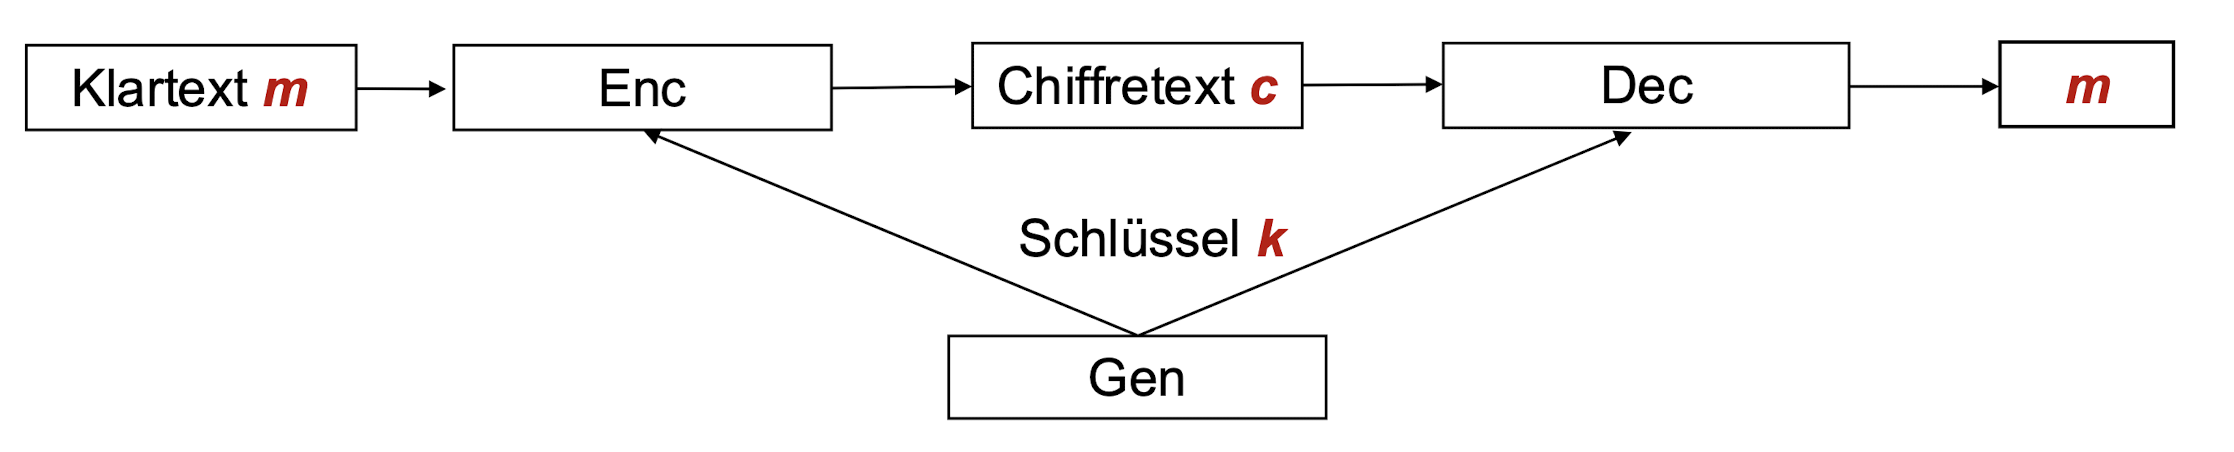
\includegraphics[width=0.7\linewidth]{/Users/lenavo/Desktop/3.Semester/Computersystemsicherheit/img/enc.png}
        \caption{Funktionale Definition}
        \label{fig:enter-label}
    \end{figure}

    \item \textbf{Gen:} generiert einen zufälligen Schlüssel $k$, der später sowohl für die Verschlüsselung als auch für die Entschlüsselung verwendet wird
    \item \textbf{Enc (Verschlüsselung):} nimmt den Klartext $m$ und Schlüssel $k$ als Eingabe und erzeugt einen Chiffretext $c$
    \item \textbf{Dec (Entschlüsselung):} nimmt den Chiffretext und denselben geheimen Schlüssel als Eingabe und stellt den ursprünglichen Text wieder her
\end{itemize}
\hl{Korrektheit:}\\
Die Entschlüsselung eines gültigen Chiffretextes resultiert in die original verschlüsselte Nachricht\\[3mm]
$Dec (k,Enc(k,m)) = m$ für alle Nachrichten $m$ und Schlüssel $k \longleftarrow Gen$\\[3mm]
\hl{Effizienz:} Verschlüsselung und Entschlüsselung sind effizient ( 1 GB/s)

\subsubsection{Sicherheitsdefinition}
\begin{itemize}
    \item \textbf{Ziel des Angreifers:} Was ist ein erfolgreicher Angriff?
    \item \hl{naive Option:} Angreifer lernt den Schlüssel $k$ nicht
    \item in der \hl{Kryptographie:} Angreifer lernt \textbf{nichts Neues} über $m$
\end{itemize}

\noindent\textbf{Angreifermodell:}
\begin{itemize}
    \item beschreibt die Fähigkeiten und Ressourcen des Angreifers
    \item Angreifer lernt \textbf{nur Chiffretext} (known ciphertext attack), z.B. durch Abhören des Kanals
    \item Angreifer lernt \textbf{Paare von Klartexten/Chiffretexten} (known plaintext/ciphertext attack), z.B. bestimmter Teil der verschlüsselten Nachricht kann bekannt sein
    \item Angreifer \textbf{wählt Klartexte und lernt zugehörige Chiffretexte} (chosen plaintext attack), z.B. Angteifer überzeugt Challenger davon, Nachrichten seiner Wahl zu verschlüsseln
\end{itemize}
\subsubsection{Sicherheitsspiel (IND-CPA)}
\begin{itemize}
    \item Sicherheit wird in der Kryptographie durch sein \textbf{Spiel} zwischen \textbf{Angreifer} und \textbf{Challenger} definiert
\end{itemize}
\begin{figure}[h]
    \centering
    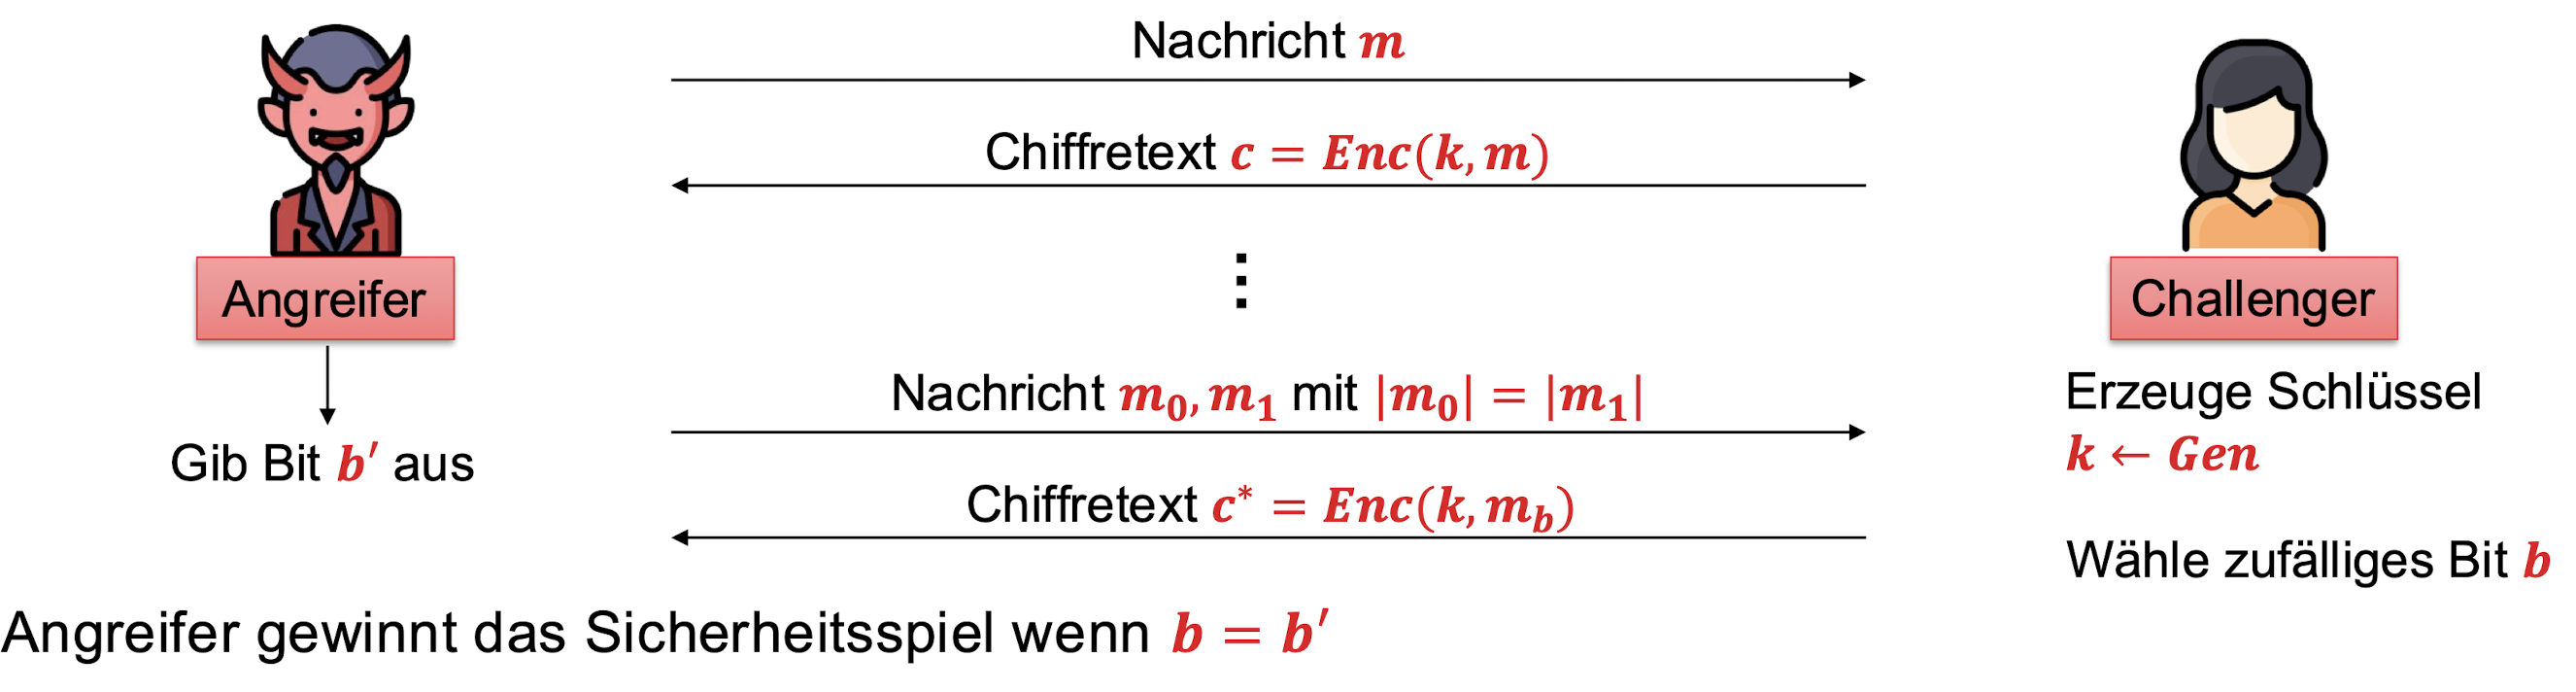
\includegraphics[width=0.7\linewidth]{/Users/lenavo/Desktop/3.Semester/Computersystemsicherheit/img/sich.png}
    \caption{Sicherheitsspiel}
    \label{fig:enter-label}
\end{figure}
\textbf{\hl{Sicherheit:}}\\[2mm] Symmetrische Chiffre ist \textbf{IND-CPA sicher}, falls alle \textbf{effizienten} Angreifer das Sicherheitsspiel maximal mit der Wahrscheinlichkeit $\approx \frac{1}{2}$ gewinnen können\\[3mm]
\textbf{Was bedeutet effizient?}
\begin{itemize}
    \item \hl{effizient:} Laufzeit \textbf{polynomiell} in der Schlüssellänge
    \item \hl{nicht effizient:} Laufzeit \textbf{exponentiell} in der Schlüssellänge
\end{itemize}

\subsubsection{Bietet IND-CPA die stärkste Sicherheit?}
\begin{itemize}
    \item Nein, es gibt noch stärkere
    \item IND-CPA bietet grundlegenden Schutz gegen \hl{passive Angriffe} (nur Zugriff auf Verschlüsselungen)
    \item Gefahr : \hl{Chosen Ciphertext Angriff}
    \begin{itemize}
        \item Angreifer hat auch Zugang zu \textbf{Entschlüsselung} von (bestimmten) Chiffretexten
        \item Angreifer kann diese Informationen nutzen, um \textbf{sensitive Informationen} zu erlangen
    \end{itemize}

    \item Beispiel: \textbf{Padding Orakel Angriff}
    \begin{itemize}
        \item Angreifer kann durch gezielte \textbf{Entschlüsselungsanfragen} Informationen über den Klartext gewinnen
    \end{itemize}
\end{itemize}

\subsubsection{Stärkere Sicherheit: IND-CCA}
\begin{figure}[h]
    \centering
    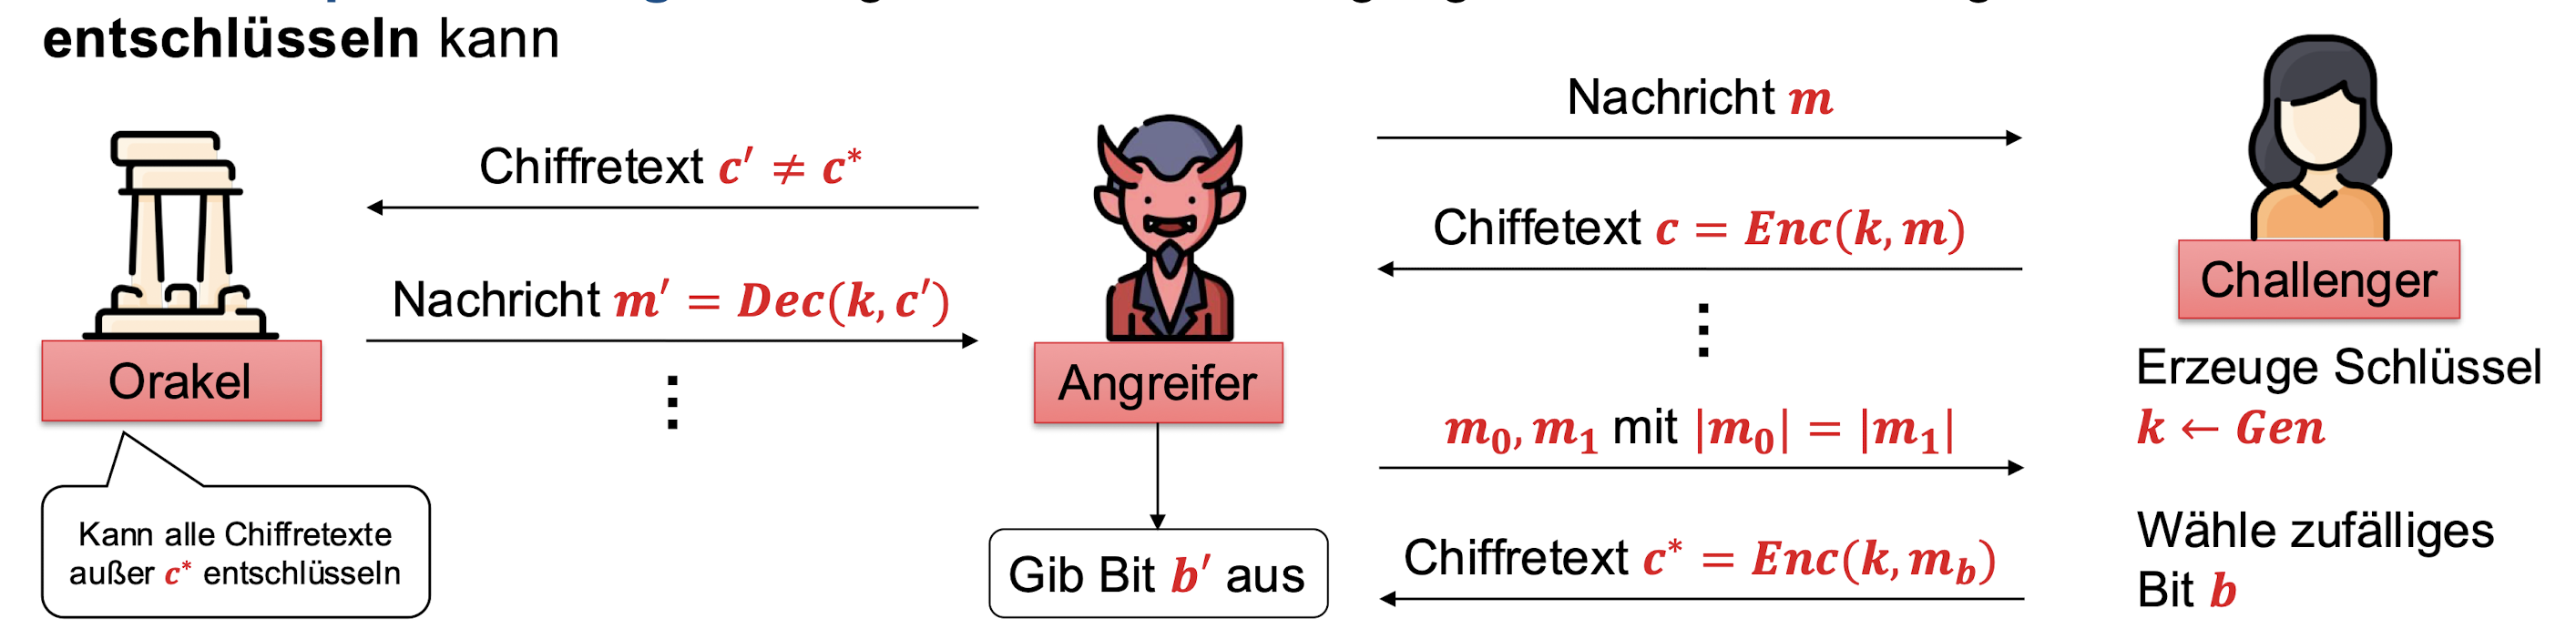
\includegraphics[width=0.7\linewidth]{/Users/lenavo/Desktop/3.Semester/Computersystemsicherheit/img/ind-cca.png}
    \caption{Sicherheitsspiel}
    \label{fig:enter-label}
\end{figure}
\begin{itemize}
    \item \textbf{Chosen Ciphertext Angriff}
    \item geht einen Schritt weiter als IND-CPA und schützt auch vor Angreifern, die zusätzlich die Möglichkeit haben, \textbf{bestimmte Chiffretexte zu entschlüsseln}
\end{itemize}
\subsubsection{Unterschied zwischen IND-CPA und IND-CCA}
\begin{itemize}
    \item \hl{IND-CPA Sicherheit:}
    \begin{itemize}
        \item schützt vor Angriffen, bei denen Angriefer \textbf{Verschlüsselungen} seiner Wahl erzeugen kann
        \item reicht nicht aus, wenn Angreifer auch \textbf{Zugriff auf Entschlüsselungen} hat
    \end{itemize}

    \item \hl{IND-CCA Sicherheit:}
    \begin{itemize}
        \item stärkere Sicherheit
        \item schützt selbst dann, wenn Angreifer zusätzlich \textbf{Entschlüsselungen anfordern} kann (außer dem zu entschlüsselnden Chiffretext)
    \end{itemize}

    \item \hl{Fazit}
    \begin{itemize}
        \item \hl{IND-CCA Sicherheit ist notwendig}, wenn Angreifer auf \textbf{Entschlüsselungsoperationen zugreifen kann}
    \end{itemize}
\end{itemize}

\noindent\textbf{Wie zeigen wir (Un-)sicherheit?}
\begin{itemize}
    \item \hl{Unsicheres Verfahren}
    \begin{itemize}
        \item konstruiere effizienten Angreifer, der mit mit Wahrscheinlichkeit signifikant größer als $\frac{1}{2}$
    \end{itemize}

    \item \hl{Sicheres Verfahren:}
    \begin{itemize}
        \item Zeige, dass \textbf{alle Angreifer} das Sicherheitsspiel mit Wahrscheinlichkeit $\approx \frac{1}{2}$ gewinnen
        \item Reduktionsbeweis auf Annahmen
    \end{itemize}
\end{itemize}

\subsection{One-Time-Pad Verschlüsselung}
\textbf{Wiederholung: XOR}
\begin{figure}[h]
    \centering
    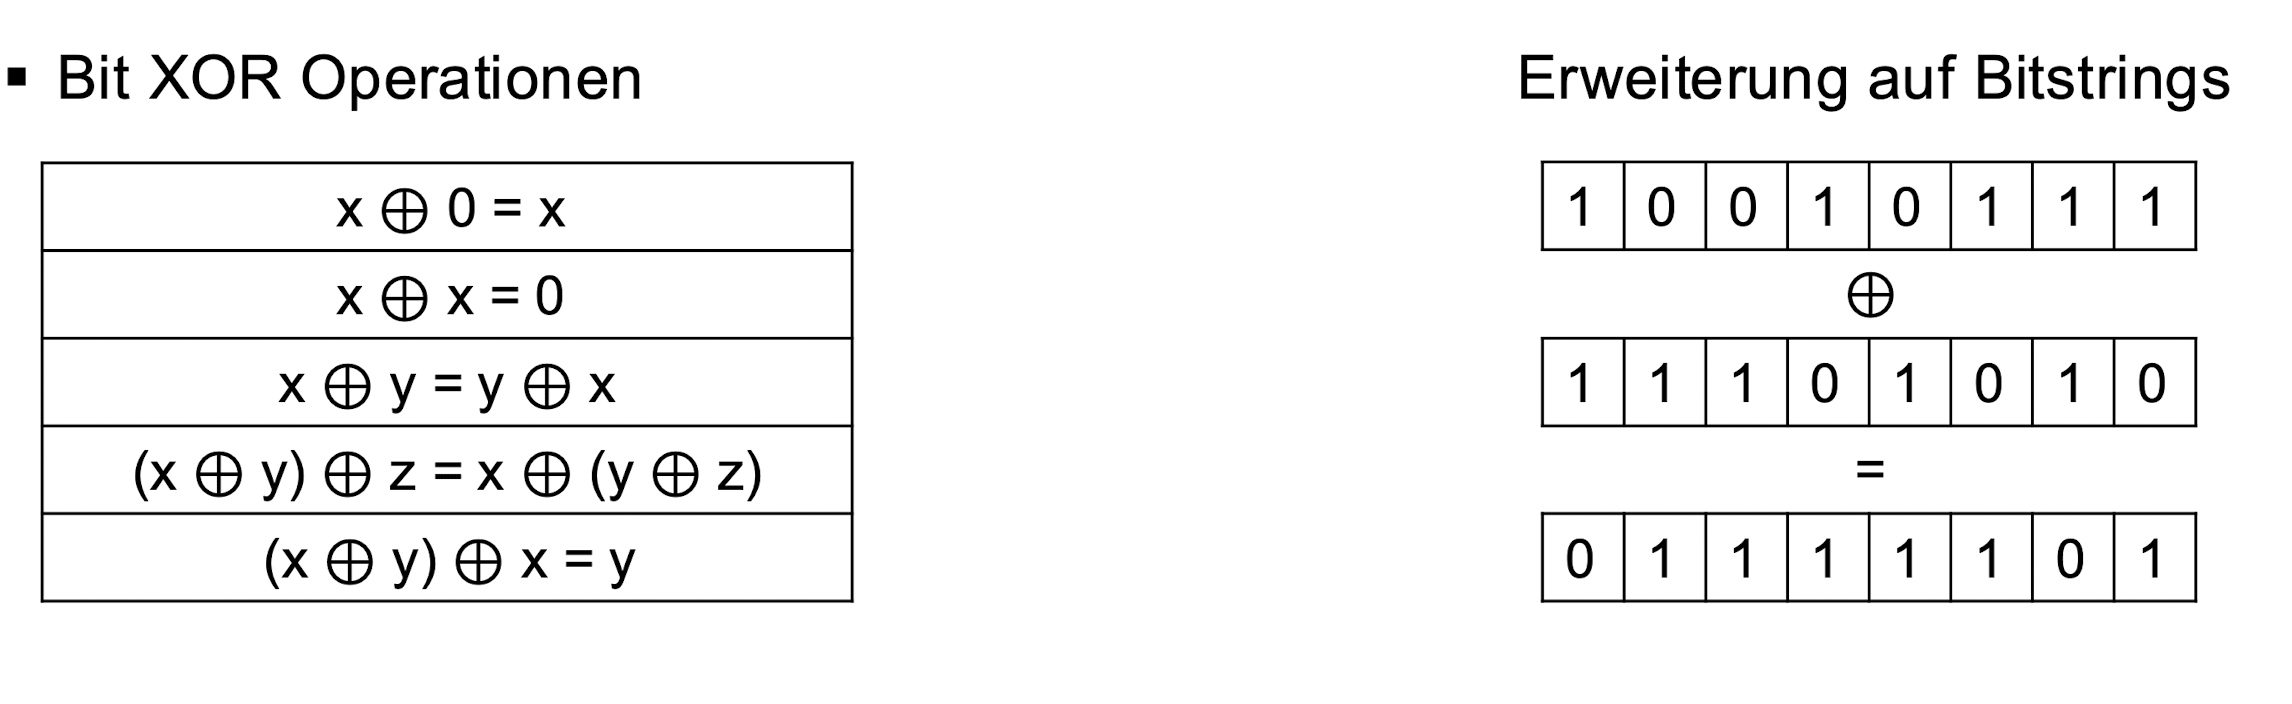
\includegraphics[width=0.7\linewidth]{/Users/lenavo/Desktop/3.Semester/Computersystemsicherheit/img/xor.png}
    \caption{XOR}
    \label{fig:enter-label}
\end{figure}
\subsubsection{One-Time-Pad}
\begin{itemize}
    \item auch häufig \textbf{Vernam-Chiffre} genannt
    \item symmetrisches Verschlüsselungsverfahren
    \item zur Verschlüsselung von \textbf{Bitstrings der Länge $n$}
\end{itemize}
\hl{Funktionsweise}
\begin{itemize}
    \item \hl{Gen:} in zufälliger \textbf{Schlüssel k} wird aus der Menge $\{0,1\}^n$ erzeugt, wobei $n$ die Länge des Klartextes m ist
    \begin{itemize}
        \item Schlüssel muss mindestens so lang wie der Klartext sein und darf nur einmal verwendet werden
    \end{itemize}
    \hl{Enc:} Verschlüsselung erfolgt durch eine \textbf{XOR-Operation} zwischen dem \textbf{Klartext m} und dem \textbf{Schlüssel k}\\[2mm]
        $\text{Enc}(k, m) = k \oplus m$ \qquad $\Longrightarrow$ Ergebnis ist der \textbf{Chiffretext c}


    \item \hl{Dec:} um den Chiffretext zu \textbf{entschlüsseln} wird erneut eine \textbf{XOR-Operation} zwischen dem \textbf{Chiffretext c} und dem \textbf{Schlüssel k} durchgeführt\\[2mm]
        $ \text{Dec}(k, c) = k \oplus c $

    
    \item da bein XOR die Operation \textbf{invertierbar ist ($x \oplus x  = 0$)}, erhält man den ursprünglichen Klartext zurück.
\end{itemize}

\subsubsection{Sicherheit}
\begin{itemize}
    \item beschränktes Sicherheitsspiel: Angriefer erhält \textbf{keinen Zugriff auf Chiffretexte}
    \item Angreifer gewinnt das Sicherheitsspiel, wenn $b = b'$
    \item Analyse ergibt: Perfekte Sicherheit - $c*$ gibt keine Information über $m_b$ preis
\end{itemize}

\begin{figure}[h]
    \centering
    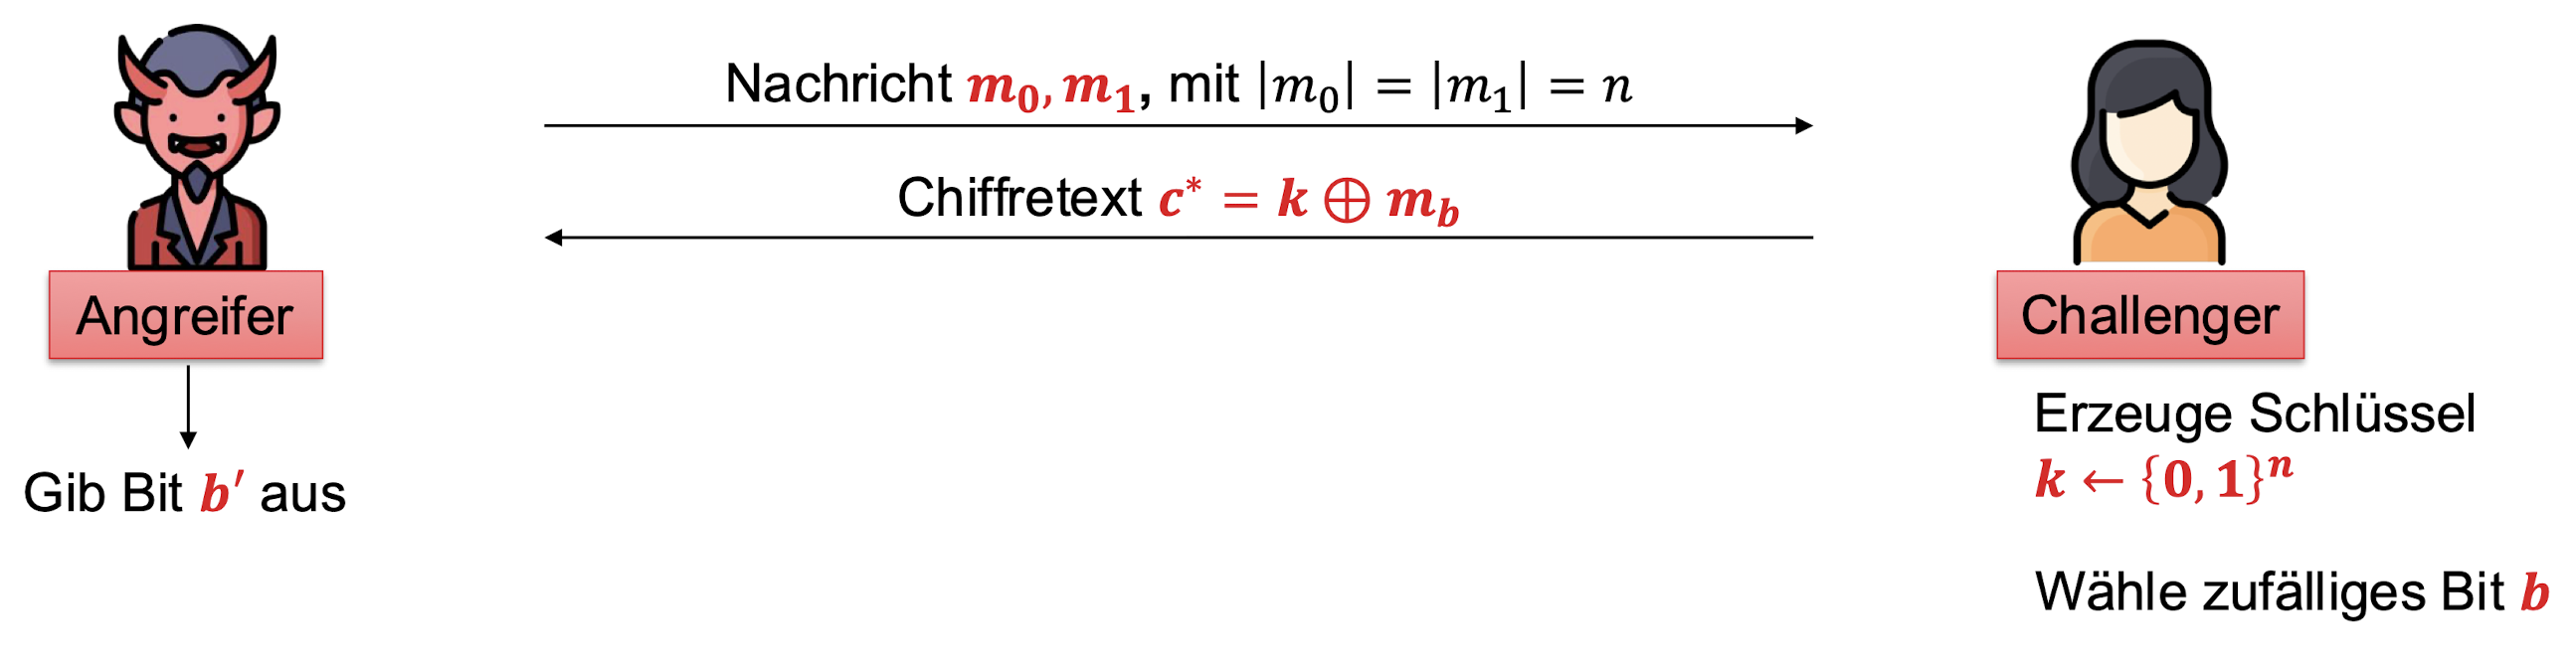
\includegraphics[width=0.7\linewidth]{/Users/lenavo/Desktop/3.Semester/Computersystemsicherheit/img/sich-ott.png}
    \caption{beschränktes Sicherheitsspiel}
    \label{fig:enter-label}
\end{figure}

\subsubsection{Schlüssel nur einmal verwenden}
\begin{figure}[h]
    \centering
    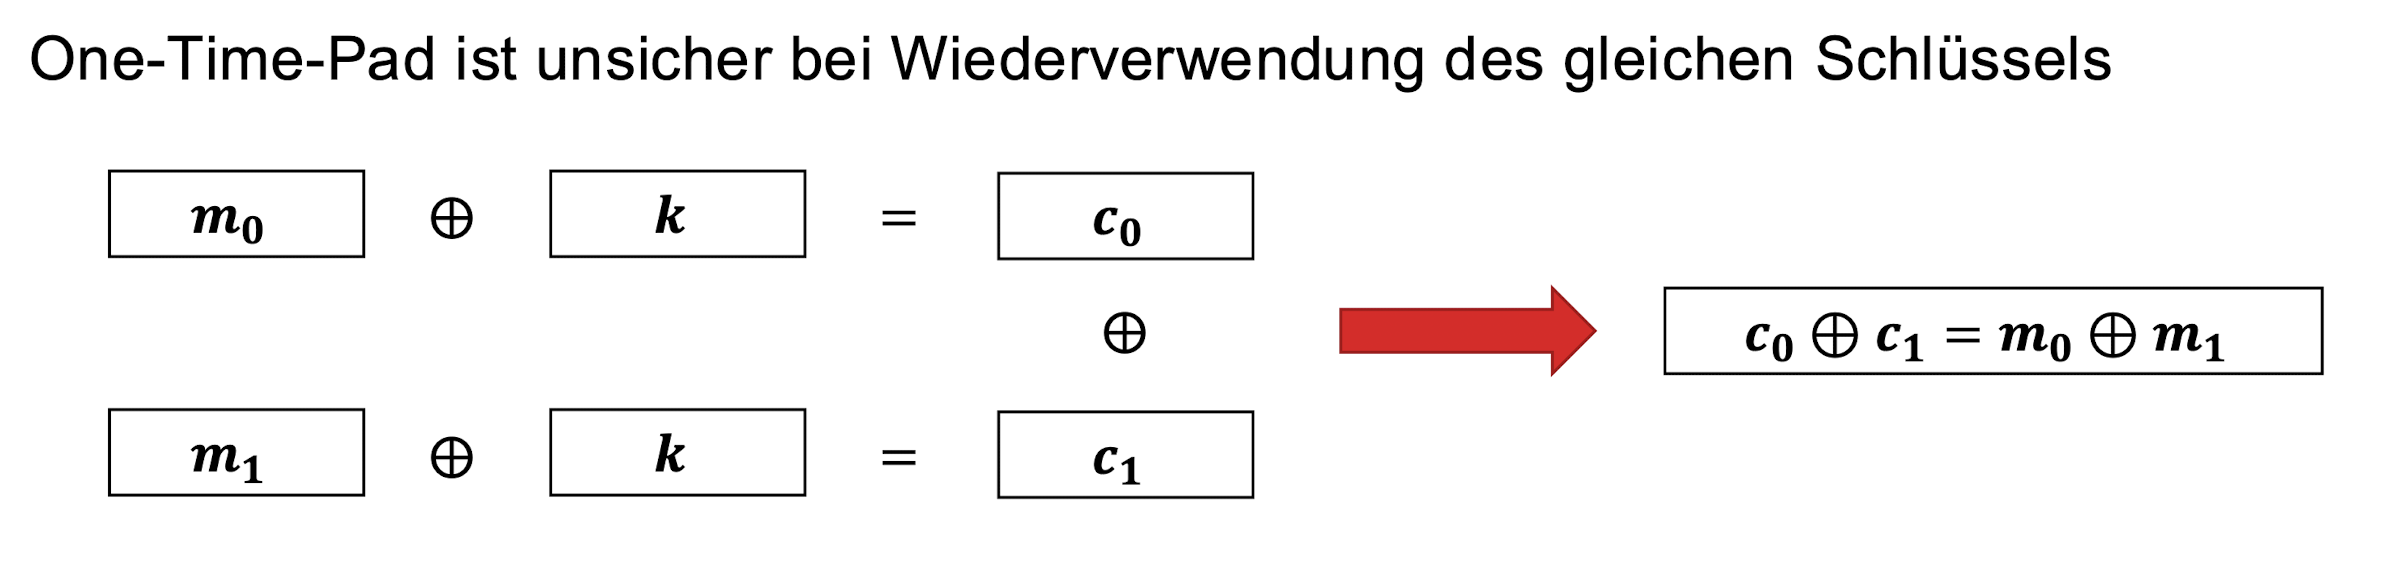
\includegraphics[width=0.7\linewidth]{/Users/lenavo/Desktop/3.Semester/Computersystemsicherheit/img/ott-key.png}
    \caption{One-Time-Pad Schlüssel nur einmal verwenden}
    \label{fig:enter-label}
\end{figure}

\begin{itemize}
    \item Lernen des XORs kann nützliche Informationen preisgeben
    \item z.B. welche Bits von $m_0$ und $m_1$ gleich sind
    \item wenn $m_0$ bekannt ist, dann ist auch $m_1$ bekannt (und vice versa)
    \item \textbf{Moral:} zur Verschlüsselung jeder Nachricht muss ein neuer zufälliger Schlüssel gewählt werden
\end{itemize}

\subsubsection{Venona-Projekt: Risiken von One-Time-Pads}
\begin{itemize}
    \item \textbf{Venona-Projekt (1943-1980)}
    \begin{itemize}
        \item \hl{Ziel:} Entschlüsselung sowjetischer Kommunikation durch USA und Großbritannien
        \item Sowjetische Nachrichten wurden mit \hl{One-Time-Pads verschlüsselt}
        \item Fehler: Schlüssel wurden unter Zeitdruck \hl{mehrfach verwendet}
    \end{itemize}

    \item \textbf{Risiken von One-Time-Pads}
    \begin{itemize}
        \item \hl{Mehrfachnutzung von Schlüsseln:} Führt dazu, dass Angreifer durch XOR der Chiffretexte Informationen über die Klartexte gewinnen können
        \item US-Geheimdienste nutzten diesen Fehler, um sowjetische Nachrichten zu entschlüsseln
    \end{itemize}

    \item \textbf{Lektion:} One-Time-Pad ist nur sicher, wenn jeder \textbf{Schlüssel einmalig} verwendet wird
\end{itemize}

\subsubsection{Nachteile von One-Time-Pad}
\begin{enumerate}
    \item Schlüssel ist \hl{so lang wie Nachricht}
    \begin{itemize}
        \item für große Mengen von Daten müssen \textbf{lange zufällige Schlüssel} gespeichert und ausgestauscht werden
        \item gute Zufälligkeit zu erzeugen, ist sehr aufwendig
    \end{itemize}


    \item Schlüssel kann \hl{nur einmal benutzt} werden
    \begin{itemize}
        \item mehrfache Verwendung kann etwa über Klartexte preisgeben
        \item für viele Nachrichten benötigt man \hl{viele Schlüssel}
    \end{itemize}


    \item Sicheheit im \hl{beschränkten Angreifermodell}
    \begin{itemize}
        \item Chiffretext-Only Angriffe
    \end{itemize}
\end{enumerate}
\section{Übung 1}
\subsection{Aufgabe 1: Wissensfragen}
\begin{enumerate} [label=(\alph*)]
    \item Beschreiben Sie die Unterschiede zwischen Safety und Security.
    \begin{itemize}
        \item \textbf{Safety (Betriebssicherheit)}
        \begin{itemize}
            \item Schutz gegen Fehler/Unfälle
            \item Fehler meist unbeabsichtigt
            \item mögliche Gegenmaßnahmen: Verifikation und Testen
        \end{itemize}

        \item \textbf{Security (Angriffssicherheit)}
        \begin{itemize}
            \item Schutz gegen worst-case-Angreifer
            \item meist Schadabsicht
            \item Verifikation und Testen hilft wenig
        \end{itemize}
    \end{itemize}

    \item Nennen und beschreiben Sie drei Sicherheitseigenschaften.
    \begin{itemize}
        \item \hl{Vertraulichkeit} (Angreifer kann Nachricht nicht lernen)
        \item \hl{Anonymität} (Eigenschaft, dass eine Person oder Gruppe nicht identifiziert werden kann)
        \item \hl{Integrität} (Angreifer kann Nachricht nicht ändern, ohne dass Änderung erkannt wird)
        \item \hl{Authentizität} (Angreifer kann nicht behaupten, dass eine Nachricht von Alive kam, die diese nicht gesendet hat)
        \item \hl{Verfügbarkeit} (Eigenschaft eines Systems Zugriff für autorisierte Benutzer auf Daten und Dienste zu erlauben)
    \end{itemize}

    \item Beschreiben Sie das Sicherheitsprinzip der fail-safe Standards. Geben Sie ein
    Beispiel an.\\[2mm]
    Dieses Prinzip sorgt dafür, dass ein System bei einem Ausfall oder einer Anomalie in einen Zustand übergeht,
der den geringstmöglichen Schaden verursacht.\\[2mm]
Beispiel: mechanisches Zugsignal (aus VL)

    \item Was sagt das Kerckhoffs’sche Prinzip aus?\\[2mm]
    Ein Kryptoverfahren soll sicher bleiben, selbst wenn der Angreifer den Kryptoalgorithmus kennt. Die Sicherheit des Kryptoverfahrens beruht auf der Geheimhaltung des Schlüssels.
\end{enumerate}

\subsection{Aufgabe 2: IND-CPA vs. IND-CCA}
\begin{enumerate} [label=(\alph*)]
    \item \textbf{Szenario 1:} Sichere Kommunikation im Web: Um Nachrichten zwischen einem
    Webbrowser und einem Webserver abzusichern, wird ein Verschlusselungsverfahren ¨
    eingesetzt. Die Kommunikation soll dabei auch gegen einen Angreifer, der die
    Kommunikationskan¨ale kontrolliert, abgesichert werden.\\[2.5mm]
    In diesem Szenario hat der Angreifer möglicherweise die Kontrolle über den Kommunikationskanal. Das bedeutet, er könnte \textbf{nicht nur Nachrichten abfangen} (passiver Angriff), sondern auch aktiv Nachrichten modifizieren oder selbst verschlüsselte Nachrichten an den Server senden (\textbf{aktiver Angriff}).
    Da die IND-CPA jedoch nur vor passiven Angriffen schützt, empfiehlt sich hier eher die \textbf{IND-CCA Sicherheit}.\\[3mm]
    Musterlösung:\\[2mm]
    Ein Angreifer, der die Kommunikationskanäle kontrolliert, kann Chiffretexte abfangen, erneut senden oder modifizieren. Der Chiffretext wird dabei vom Empfänger entschlüsselt und der Empfänger führt mögliche Aktionen aus. In diesem Szenario ist IND-CPA Sicherheit nicht ausreichend und wir brauchen IND-CCA Sicherheit des Verschlüsselungsverfahren. Der Empfänger stellt in diesem Szenario eine Art Entschlüsselungsorakel dar. Auch wenn der Empfänger die entschlüsselte Nachricht nicht an den Angreifer zurück schickt, kann der Angreifer möglicherweise Informationen aus den Aktionen des Empfängers ableiten.(z.B. der Webserver führt eine Transaktion aus). Um einen solchen Angriff zu verhindern, benötigt es eine stärkere Sicherheit als IND-CPA Sicherheit.
    \item\textbf{Szenario 2:} Data at Rest: In einem Unternehmen werden sensible Daten auf einer Festplatte gespeichert. Diese Informationen sollen durch ein Verschlüsselungsverfahren
    abgesichert werden, sodass selbst bei einem Diebstahl der Festplatte die Daten geheim bleiben.\\[2mm]
    Musterlösung:\\[2mm]
    In diesem Szenario ist IND-CPA Sicherheit ausreichend. Sollte ein Angreifer im Besitz einer Festplatte kommen, dann hat er keinen Zugriff auf ein Entschlüsselungsorakel (Unter der Annahme, dass der Schlüssel nicht auf der Festplatte gespeichert ist).
    Der Angreifer kann lediglich versuchen die Klartexte zu erraten oder andere Online-Angriffe wie einen Bruce-Force-Angriff durchzuführen.

\end{enumerate}
\section{Thema 3: Symmetrische Kryptographie - Teil }
\subsection{Data Encryption Standard (DES)}
\begin{itemize}
    \item symmetrischer Verschlüsselungsalgorithmus, der in den 1970er Jahren von IBM im Auftrag des National Institute of Standards and Technology (NIST) entwickelt wurde 
    \item \textbf{Blockchiffre}, die Daten in \text{Blöcken} von \textbf{64 Bit} verschlüsselt und entschlüsselt
    \item \textbf{Blocklänge}: \hl{n=64} Bits
    \item \textbf{Schlüssellänge:} \hl{k=56} Bits
\end{itemize}
\textbf{Verschlüsselung und Entschlüsselung}
\begin{itemize}
    \item Verschlüsselung erfolgt mit einem Schlüssel $K \in \{0,1\}^{56}$ und einer Nachricht $M \in\{0,1\}^{64}$
    \item das Ergebnis ist ein Chiffrat $C \in \{ 0,1\}^{64}$
    \item die Entschlüsselung funktioniert ähnlich, wobei derselbe Schlüssel K verwendet wird, um das Chiffrat C wieder in die ursprüngliche Nachricht M zu konvertieren
\end{itemize}
\newpage
\begin{figure}[h]
    \centering
    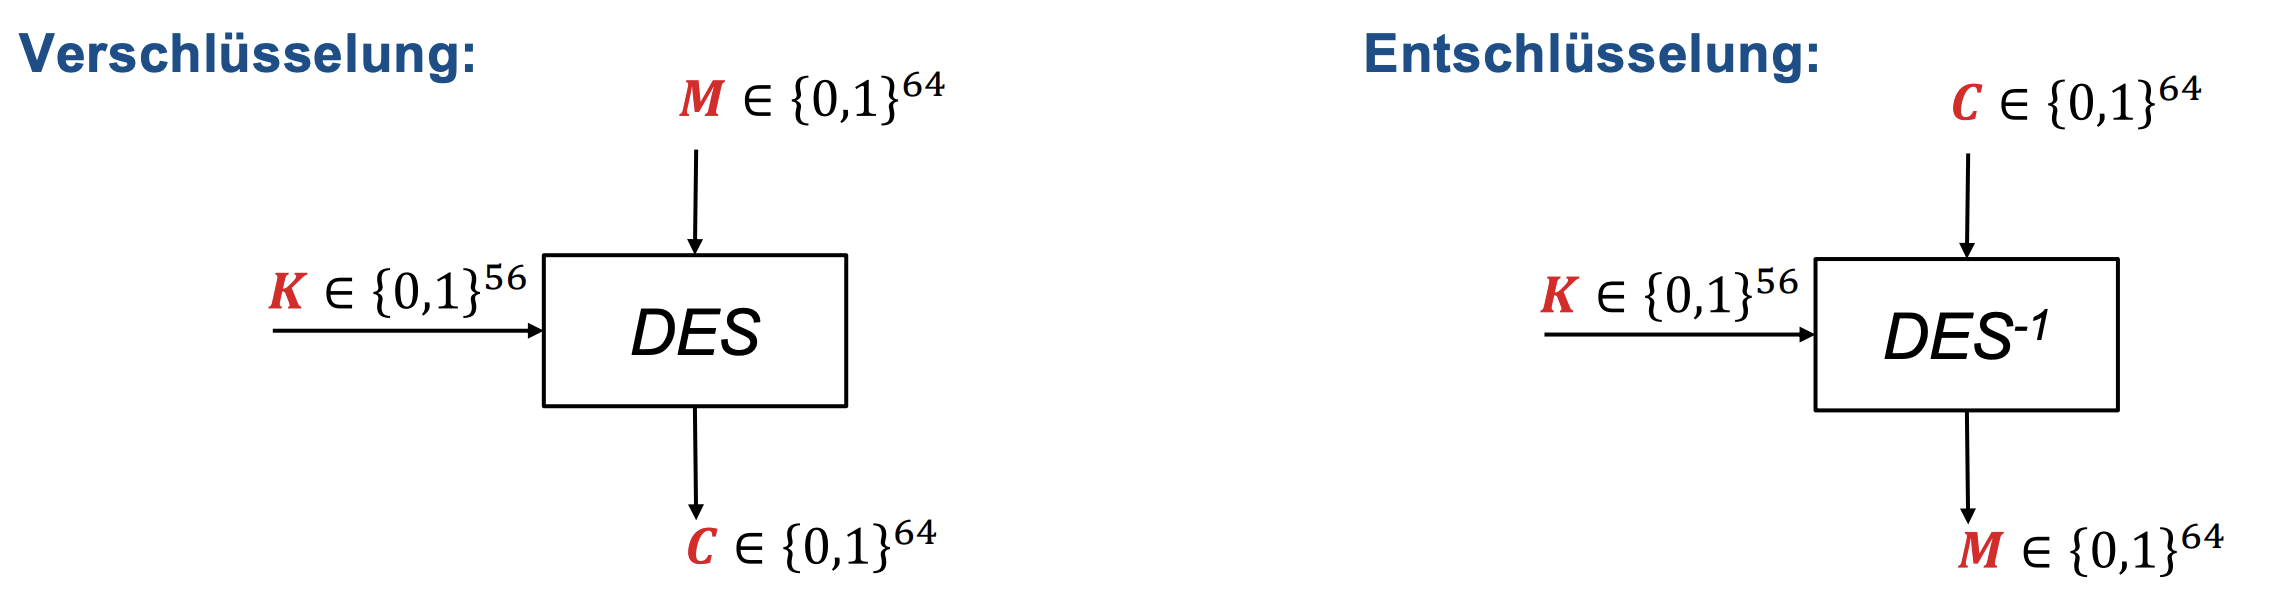
\includegraphics[width=0.7\linewidth]{/Users/lenavo/Desktop/3.Semester/Computersystemsicherheit/img/Des.png}
    \caption{Des}
    \label{fig:enter-label}
\end{figure}

\subsubsection{DES: Angriffe}
\hl{Theoretische Angriffe:}
\begin{itemize}
    \item \textbf{Differenzielle Kryptoanalyse}
    \item \textbf{Lineare Kryptoanlyse}
    \item DES bietet Schutz gegen Differenzielle Kyptoanalyse
    \item \textbf{Hauptschwachpunkt:} kurzer Schlüssel (nur 56 Bits)
    \begin{itemize}
        \item Brute-Force Angriff ist möglich
        \item DES Cracker: bricht DES in wenigen Tagen (in 1988)
        
    \end{itemize}
    \item \textbf{Erweiterungen:} Mehrfachanwendung von DES zur Verlängerung des Schlüssels (z.B. Triple DES)
\end{itemize}

\subsubsection{Triple-DES}
\begin{itemize}
    \item DES-Algorithmus wird dreimal hintereinander auf einen Datenblock angewendet, um die Sicherheit zu erhöhen
    \item dabei werden \textbf{drei 56-Bit-Schlüssel} verwendet, was zu einer \hl{nominalen Schlüssellänge} von \textbf{168 Bits} führt
\end{itemize}
\textbf{Meet-in-the-Middle Angriff}
\begin{itemize}
    \item nutzt den Umstand aus, dass der Angreifer sowohl den Klartext als auch den Chiffretext kennt und durch \textbf{Berechnung von Zwischenergebnissen} den Schlüsselraum effizienter durchsuchen kann
    \item funktioniert folgendermaßen:
    \begin{enumerate}
        \item Ein Angreifer berechnet für alle möglichen Schlüssel $K_0$ das Ergebnis $X = DES(M, K_0)$, wobei $M$ die bekannte Nachricht ist ($2^{56}$ Möglichkeiten)
        \item danach berechnet er für alle möglichen Schlüssel $K_1$ das Ergebnis $Y= DES^{-1}(X,K_1)$ ($2^{56}$ $\cdot$ $2^{56}$ Möglichkeiten)
        \item schließlich berechnet er für alle möglichen Schlüssel $K_2$ das Ergebnis $Z = DES^{-1} (C, K_2)$, wobei C der bekannte Chiffretext ist
        \item Der Angreifer vergleicht nun alle Werte von $Y$ ind $Z$. Wenn eine Übereinstimmung gefunden wird, hat er potenziell den richtigen Schlüssel gefunden
    \end{enumerate}
    \item dieser Angriff reduziert den Aufwand für das Knacken von Triple-DES auf etwa $2^{112}$ Operationen anstatt der erwarteten $2^{168}$ Operationen
\end{itemize}

\subsection{Advanced Encryption Standard (AES)}
\begin{itemize}
    \item Schlüsselgröße: \textbf{128, 192} oder \textbf{256} Bit
    \item Block-Größe: \textbf{128} Bit
    \item gilt als unangebrochen: in den USA Zulassung für \textbf{höchte Geheimhaltungsstufe}
\end{itemize}
\subsubsection{Angriffe in der Praxis}
\begin{enumerate}
    \item \textbf{Seiten-Kanal-Angriffe}
    \begin{itemize}
        \item \hl{passive Angriffe}, bei denen der Angreifer \textbf{physikalische Informationen} während der Ausführung einer kryptographischen Operation beobachtet
        \item Messe die \textbf{Zeit}, die für kryptographische Operationen benötigt wird 
        \item Messe den \textbf{Stromverbrauch}
    \end{itemize}

    \item \textbf{Fehlerangriffe}
    \begin{itemize}
        \item \hl{aktive Angriffe}, bei denen der Angreifer gezielt \textbf{Fehler in den Berechnungsprozess} einführt
        \item können durch \textbf{physikalische Manipulationen}, wie Laserstrahlen, elektromagnetische Pulse oder Spannungsschwankungen verursacht werden
        \item Ziel ist es durch die \textbf{Analyse der fehlerhaften Ausgaben} Informationen über den geheimen Schlüssel zu gewinnen
    \end{itemize}
\end{enumerate}

\noindent\textbf{Blockchiffren im Einsatz}
\begin{itemize}
    \item \hl{nicht IND-CPA sicher}
    \item Nachrichten belieber Länge können nicht direkt verschlüsselt werden
    \item Merke: Deterministische Verschlüsselung kann nicht IND-CPA sicher sein
\end{itemize}


\subsection{Modes of Operation}
\begin{itemize}
    \item Ziel: Verschlüsselung von Nachrichten mit \hl{beliebiger Länge}
\end{itemize}
\begin{enumerate}
    \item \textbf{Electronic Codebook (ECB)} Modus
    \begin{itemize}
        \item nicht IND-CPA sicher
    \end{itemize}

        \item \textbf{Cipher-Block-Chaining (CBC)} Modus
        \item \textbf{Counter (CTR)} Modus
\end{enumerate}
\subsubsection{Electronic Code Book (ECB) Modus}
\begin{itemize}
    \item jeder Klartextblock wird \textbf{unabhänig} voneinander mit \textbf{demselben Schlüssel} verschlüsselt
    \item bedeutet, dass identische Klartextblöcke immer zu identischen Chiffretextblocken führen $\rightarrow$ erhebliche Schwäche
\end{itemize}
\begin{figure}[h]
    \centering
    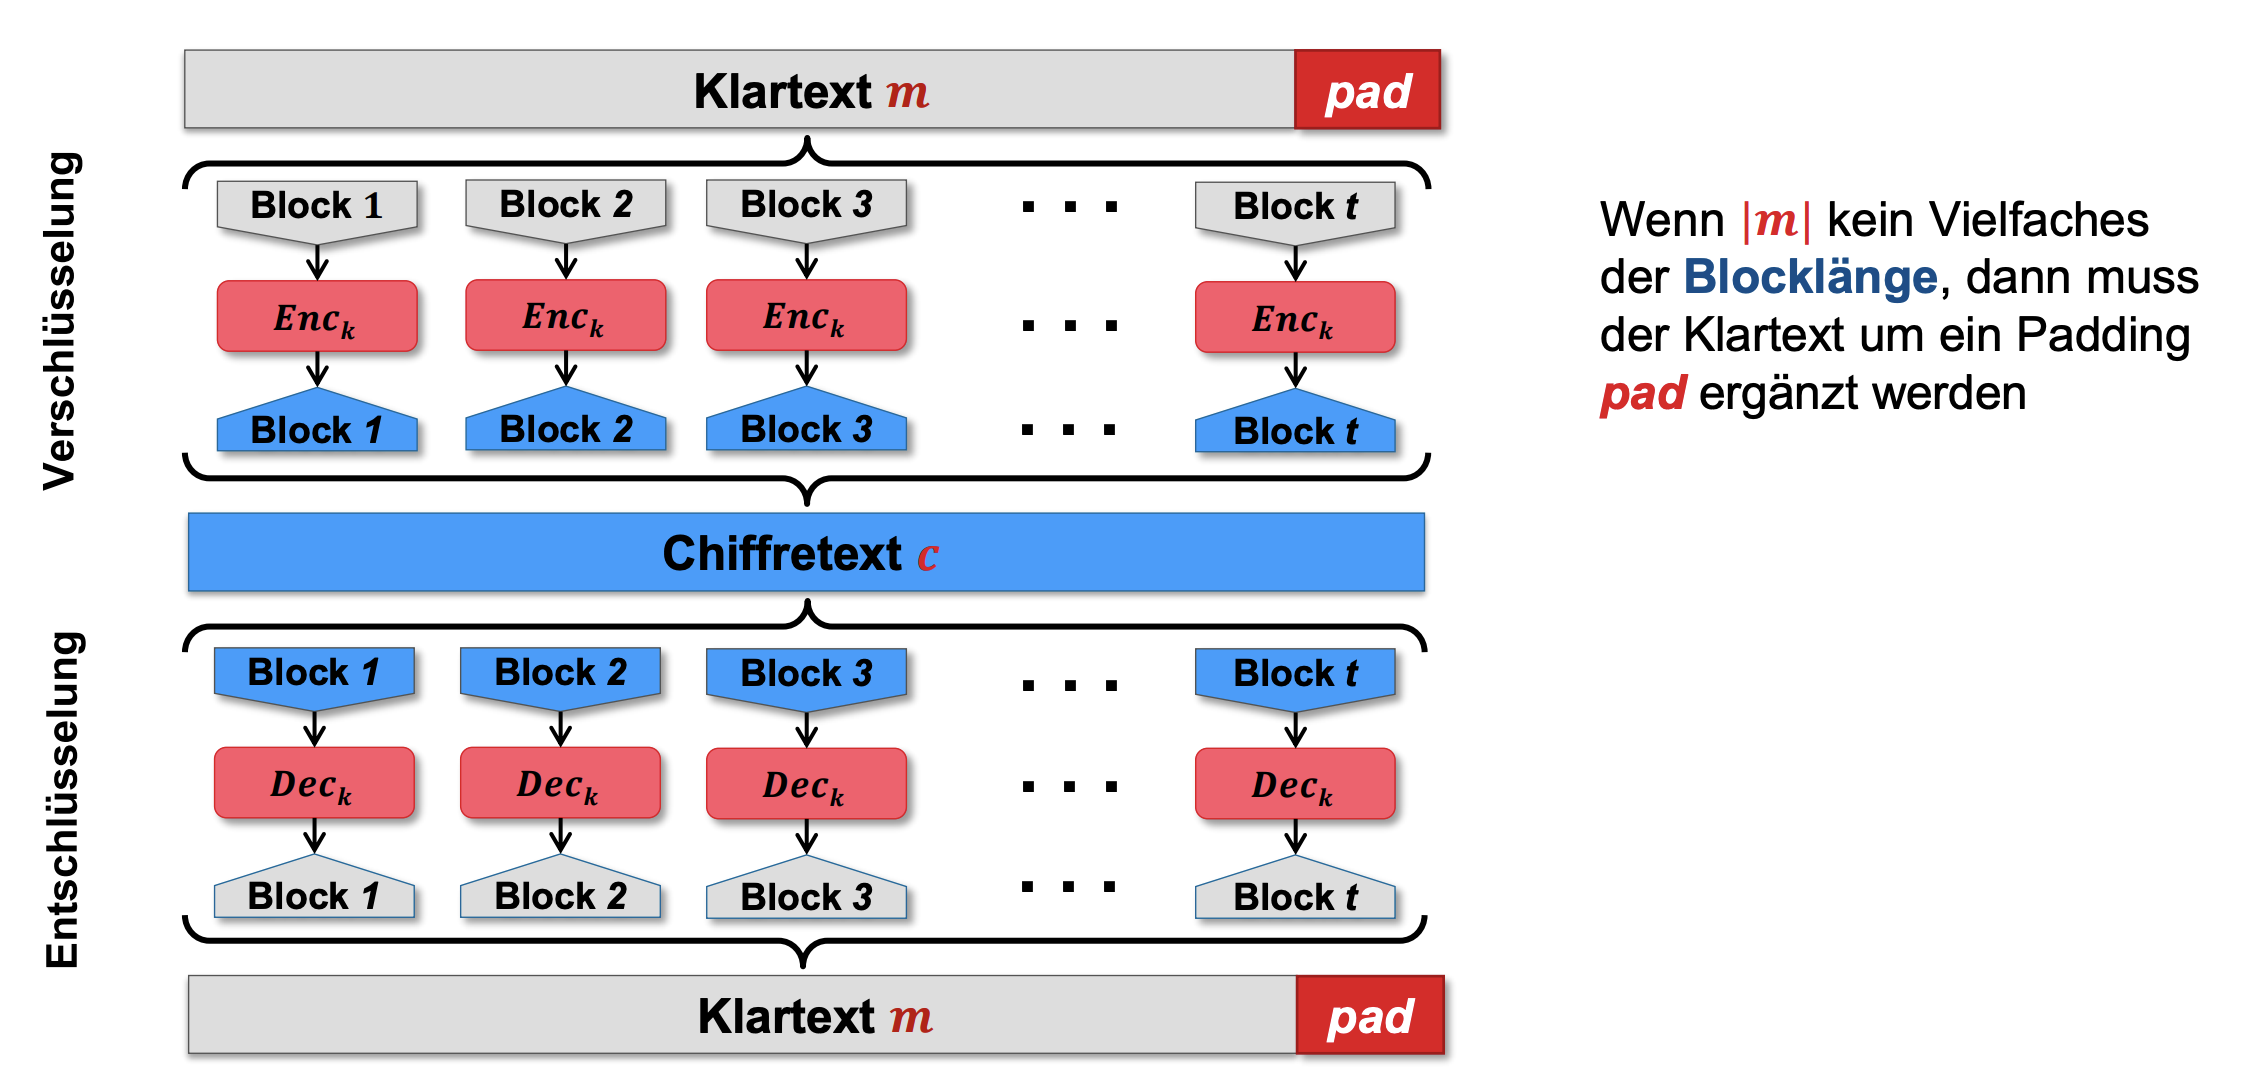
\includegraphics[width=0.6\linewidth]{/Users/lenavo/Desktop/3.Semester/Computersystemsicherheit/img/ecb.png}
    \caption{ECB-Modus}
    \label{fig:enter-label}
\end{figure}
\textbf{Funktionsweise:}
\begin{enumerate}
    \item \hl{Aufteilung des Klartextes in Blöcken}
    \begin{itemize}
        \item Klartext $m$ wird in Blöcke der Größe der Blockchiffre unterteilt
        \item wenn Länge des Klartextes $|m|$ \textbf{kein Vielfaches} der Blockgröße ist, wird der letzte Block durch \hl{Padding} (Auffüllen) ergänzt, um die Blockgröße zu erreichen
    \end{itemize}

    \item \hl{Verschlüsselung:}
    \begin{itemize}
        \item jeder Klartexttblock wird \textbf{unabhängig} voneinander mit dem \textbf{gleichen Schlüssel $k$} verschlüsselt
        \[
            c_i = Enc_k (m_i)
        \]
    \end{itemize}

    \item \hl{Entschlüsselung:}
    \begin{itemize}
        \item jeder Chiffretextblock wird unabhänig voneinander mit dem gleichen Schlüssel entschlüsselt
        \[
            m_i = Dec_k(c_i)
        \]
        \item die entschlüsselten Blöcke werden zu einem \textbf{Klartextblock kombiniert}
    \end{itemize}
\end{enumerate}
\textbf{Schwächen des ECB-Modus:}
\begin{itemize}
    \item da jeder Block unabhängig verschlüsselt wird, gibt es \textbf{keine Zufälligkeit oder Verknüpfung} zwischen den Blöcken
    \begin{itemize}
        \item führt dazu, dass ein Angreifer, der einen Teil des Klartextes kennt, leicht \hl{Rückschlüsse} auf den Chiffretext ziehen kann 
    \end{itemize}
\end{itemize}

\subsubsection{Cipher Block Chaining (CBC) Modus}
\begin{itemize}
    \item jeder Klartextblock wird vor der Verschlüsselung mit dem \textbf{vorherigen Klartextblock verknüpft}, was sicherstellt, dass gleiche Klartextblöcke nicht zu gleichen Chiffretextblocken führen
    \begin{itemize}
        \item dadurch wird eine Form der \textbf{Randomisierung} eingeführt
    \end{itemize}
\end{itemize}
\begin{figure}[h]
    \centering
    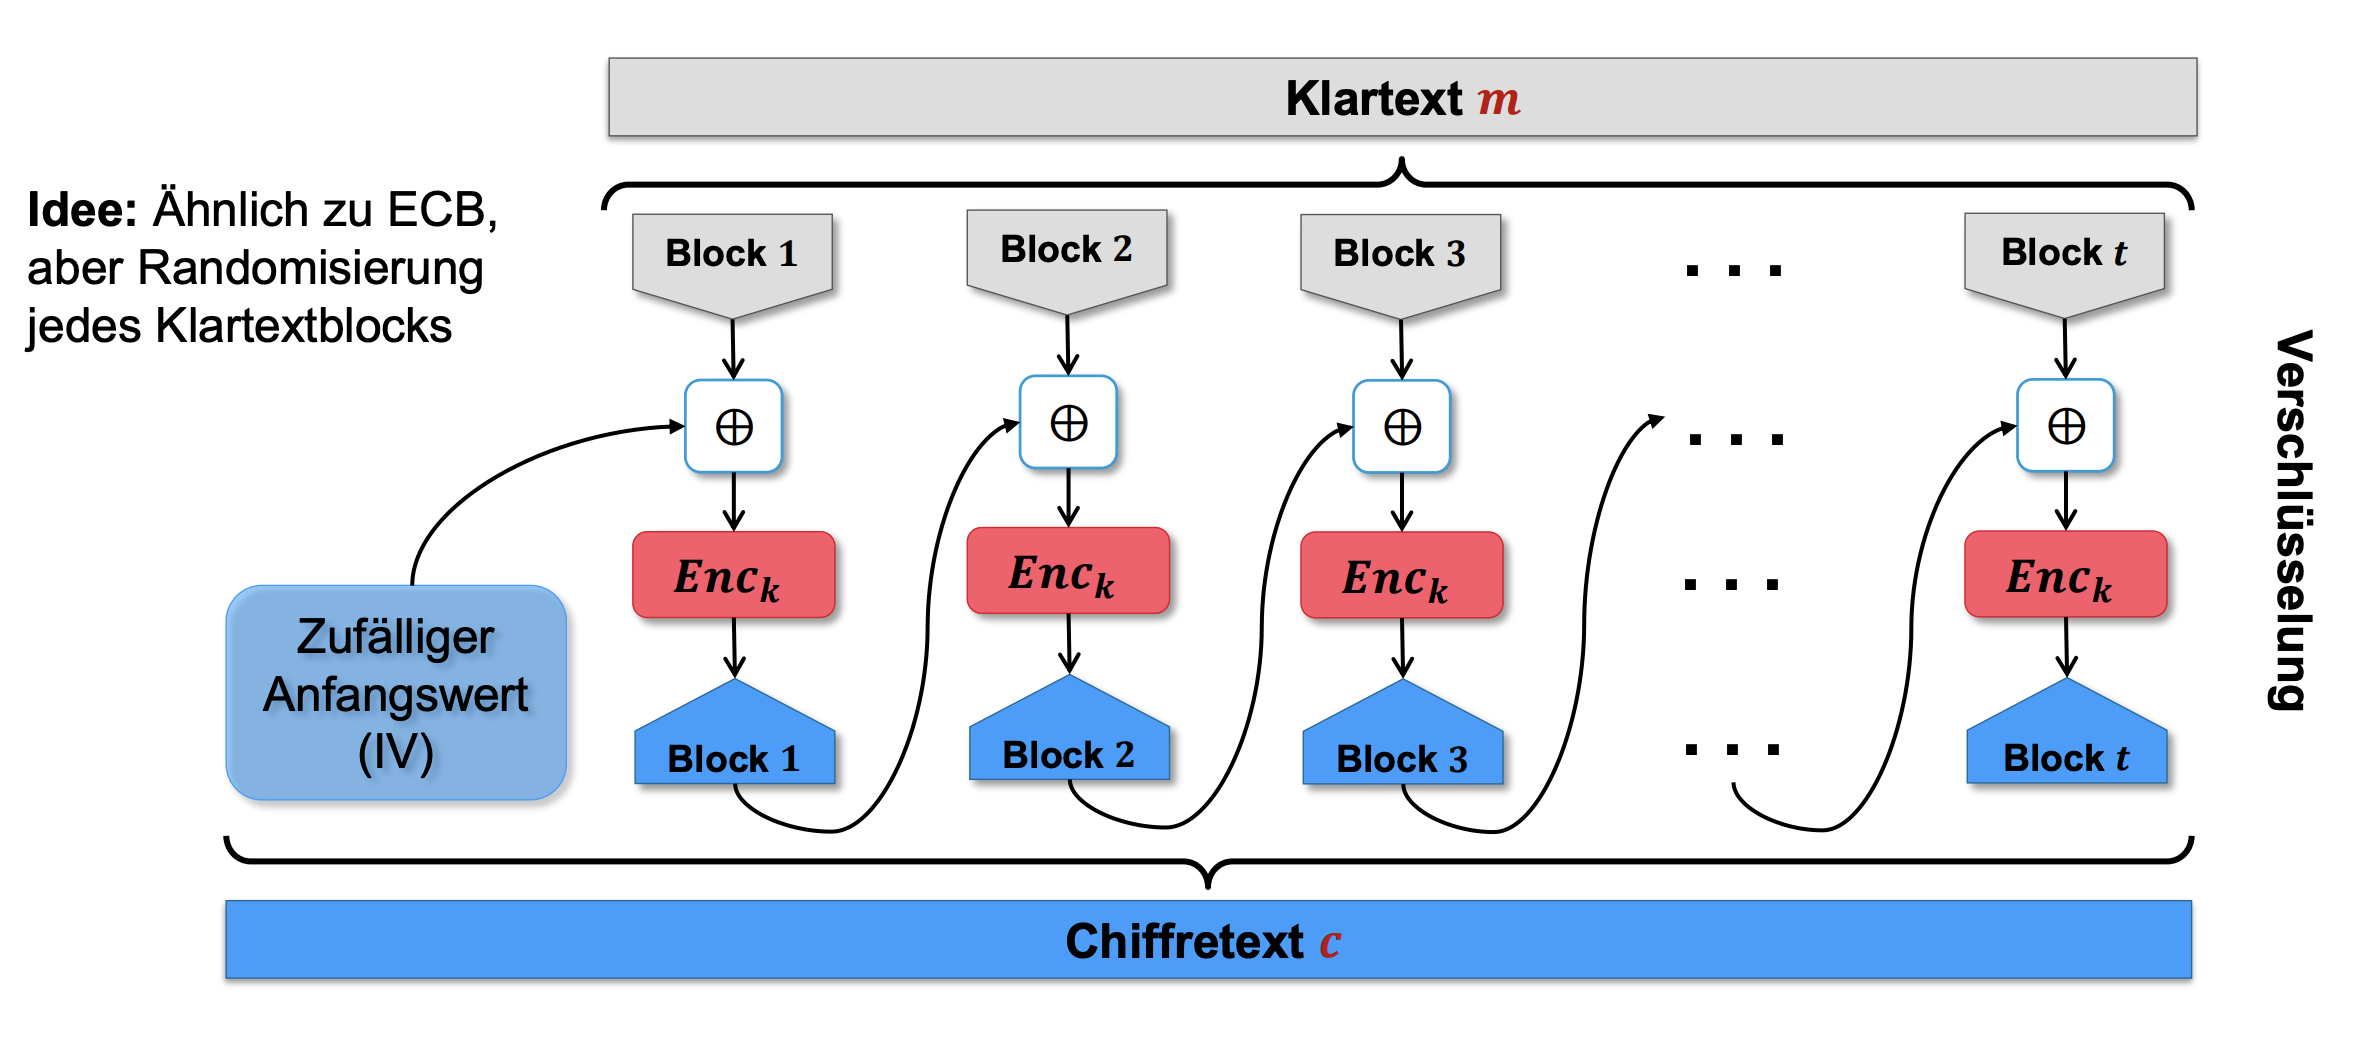
\includegraphics[width=0.6\linewidth]{/Users/lenavo/Desktop/3.Semester/Computersystemsicherheit/img/cbc1.png}
    \caption{CBC-Verschlüsselung}
    \label{fig:enter-label}
\end{figure}\newpage
\begin{figure}[h]
    \centering
    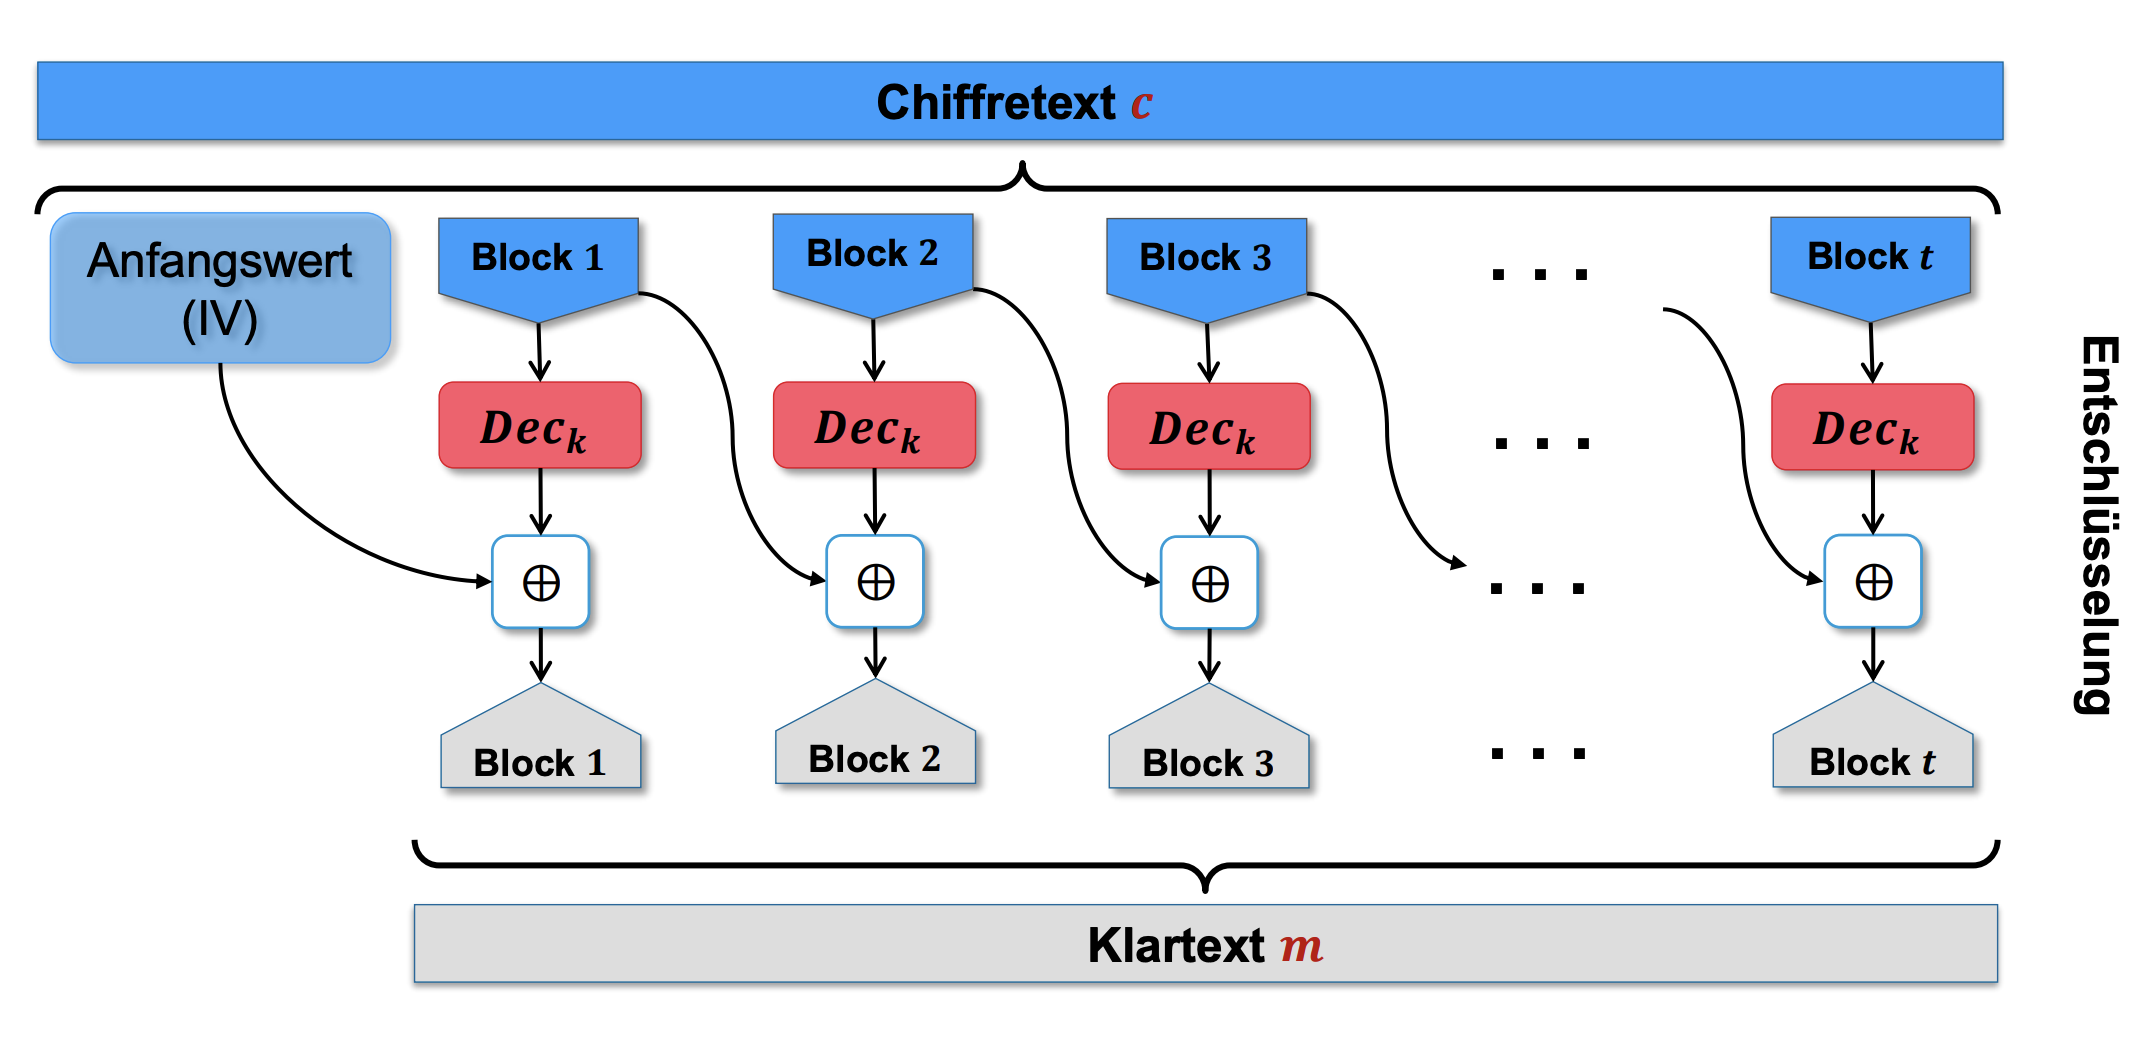
\includegraphics[width=0.6\linewidth]{/Users/lenavo/Desktop/3.Semester/Computersystemsicherheit/img/cbc2.png}
    \caption{CBC-Entschlüsselung}
    \label{fig:enter-label}
\end{figure}
\noindent\textbf{Funktionsweise des CBC-Modus:}
\begin{enumerate}
    \item \hl{Initialisierungsvektor (IV):}
    \begin{itemize}
        \item beginnt mit einem zufälligen Initialisierungsvektor, der \textbf{genau so lang ist wie ein Block}
    \end{itemize}

    \item \hl{Verknüpfung der Blöcke:}
    \begin{itemize}
        \item jeder Klartextblock wird vor der Verschlüsselung mit dem \textbf{Chiffretext des vorherigen Blocks} XOR verknüpft
    \end{itemize}

    \item \hl{Entschlüsselung:}
    \begin{itemize}
        \item jeder Chiffretext wird entschlüsselt und dann mit dem vorherigen Chiffretextblock XOR verknüpft, um den ursprünglichen Klartext wiederherzustellen
    \end{itemize}
\end{enumerate}

\noindent\textbf{CBC-Modus: Sicherheit}
\begin{itemize}
    \item ist \hl{IND-CPA sicher}, wenn er korrekt verwendet wird
\end{itemize}

\noindent\textbf{Padding Angriffe auf CBC}
\begin{itemize}
    \item Chosen-Ciphertext Angriffe können Informationen über Bits der Nachricht liefern
    \item Bitänderungen in Chiffretext Block 1 führen zu Änderungen in Klartext Block 2
    \item wenn angteifer lernt ob bei der Entschlüsselung das Padding ungültig war, können \textbf{gezielte Modifikationen} in Block 1 \textbf{Informationen} über Klartext in Block 2 liefern
\end{itemize}
\hl{Angriffsszenario:}
\begin{itemize}
    \item Angreifer hat Zugriff auf verschlüsselten Chiffretext, der im CBC-Modus erstellt wurde
    \item \textbf{kennt den Schlüssel nicht}, hat jedoch die Möglichkeit, den Chiffretext zu \textbf{modifizieren} und an ein \textbf{System zu senden}, das die Entschlüsselung durchführt
    \item System gibt Rückmeldungen darüber, ob das \textbf{Padding nach der Entschlüsselung korrekt} war (z.B. durch Fehlermeldungen)
\end{itemize}
\textbf{Sicherheit gegen Padding-Angriffe vs. IND-CPA/IND-CCA}
\begin{itemize}
    \item Sicherheit gegen Padding Angriffe ist \textbf{stärker} als IND-CPA Sicherheit 
    \begin{itemize}
        \item Bsp: CBC-Mode ist IND-CPA sicher, aber nicht gegem Padding Angriffe
    \end{itemize}

    \item im IND-CCA Spiel hat Angreifer Zugriff auf \hl{Entschlüsselungsorakel}
    \begin{itemize}
        \item kann alles, was Padding Orakel auch kann (aber noch mehr)
        \item ist mächtiger als ein Padding Orakel!
        \item IND-CCA bietet \textbf{stärkere Sicherheit}
    \end{itemize}
\end{itemize}
$\rightarrow$ Sicherheit gegen Padding Angriffe liegt \textbf{zwischen IND-CPA und IND-CCA Sicherheit}
\subsubsection{Counter Modus (CTR)}
\begin{itemize}
    \item Idee: Nutze Ausgabe der Blockchiffre als One-Time-Pad
    \item anstatt wie beim One-Time-Pad einen großen zufälligen Schlüssel zu verwenden, wird beim CTR-Modus ein \hl{Zählerwert(Counter)} verwendet
    \item dieser Zähler wird bei jeder Verschlüsselung \textbf{inkrementiert} und zusammen mit einem festen Wert verschlüsselt
\end{itemize}
\begin{figure}[h]
    \centering
    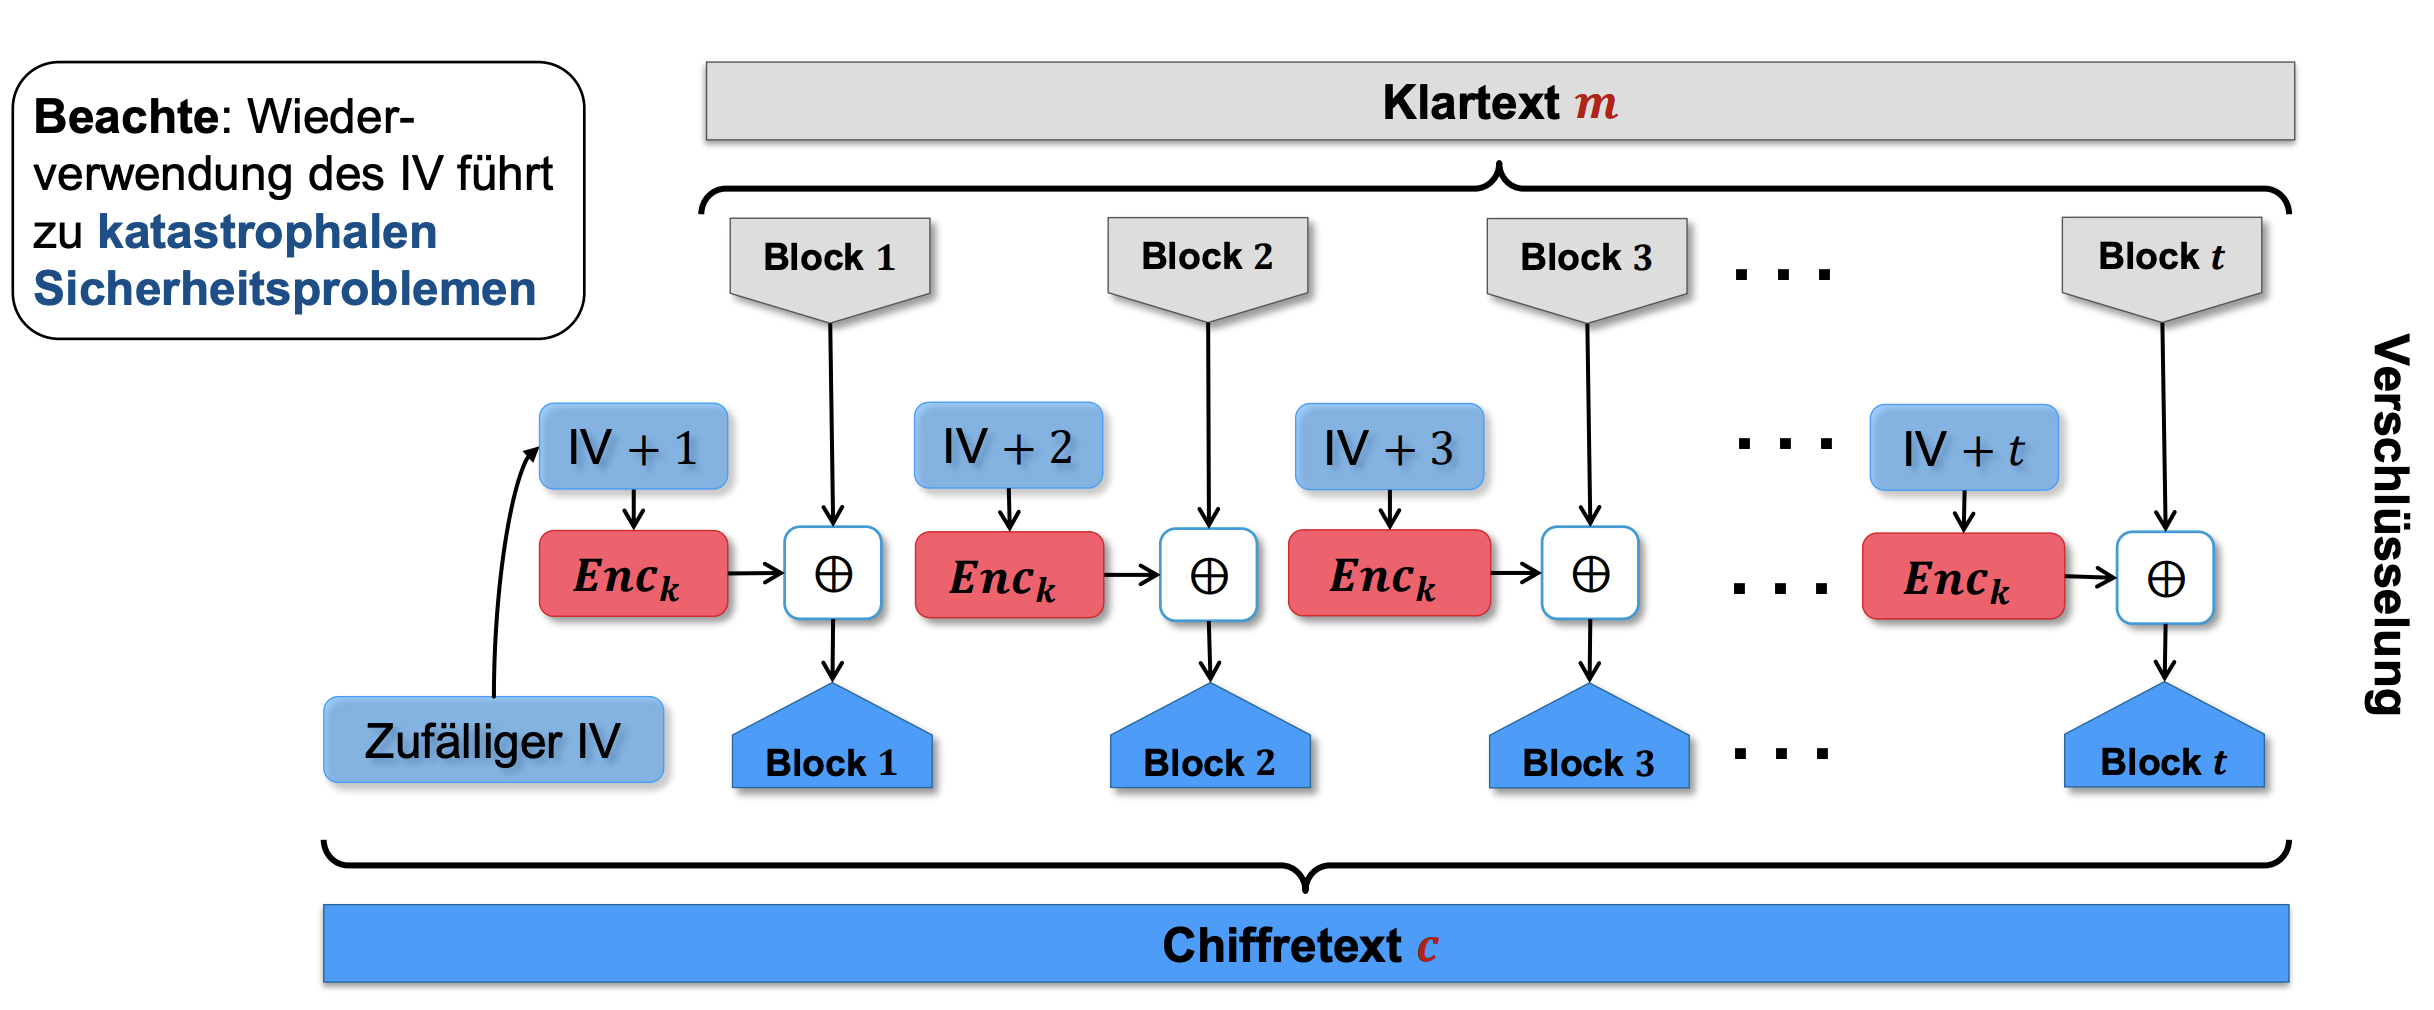
\includegraphics[width=0.6\linewidth]{/Users/lenavo/Desktop/3.Semester/Computersystemsicherheit/img/ctr.png}
    \caption{Counter Modus}
    \label{fig:enter-label}
\end{figure}
\textbf{Fehlerresistenz}
\begin{figure}[h]
    \centering
    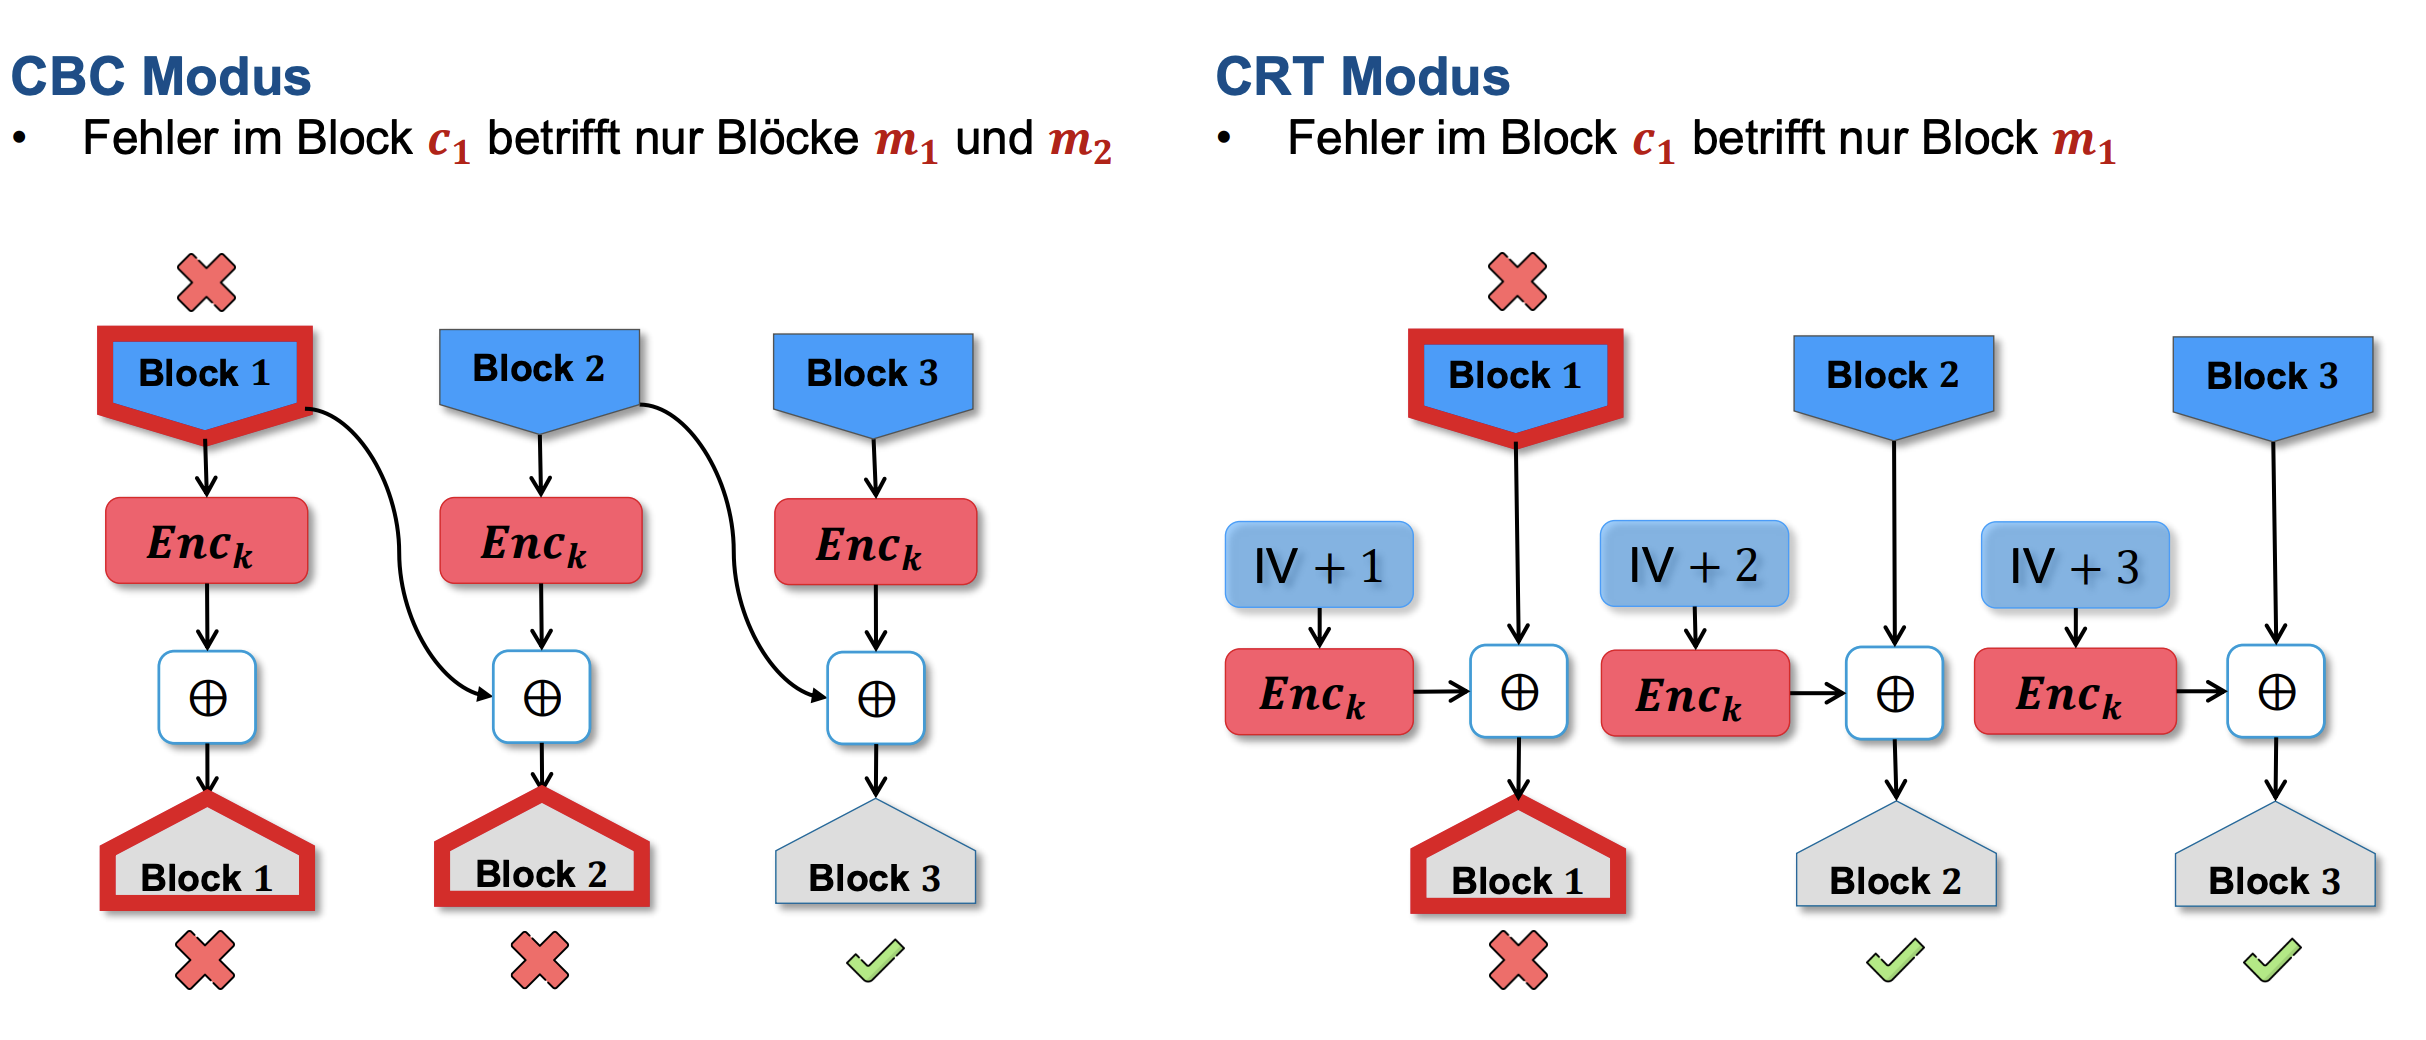
\includegraphics[width=0.7\linewidth]{/Users/lenavo/Desktop/3.Semester/Computersystemsicherheit/img/Fehlerresistenz.png}
    \caption{Fehlerresistenz}
    \label{fig:enter-label}
\end{figure}\\[2mm]
\textbf{Vergleich der Modi}
\begin{figure}[h]
    \centering
    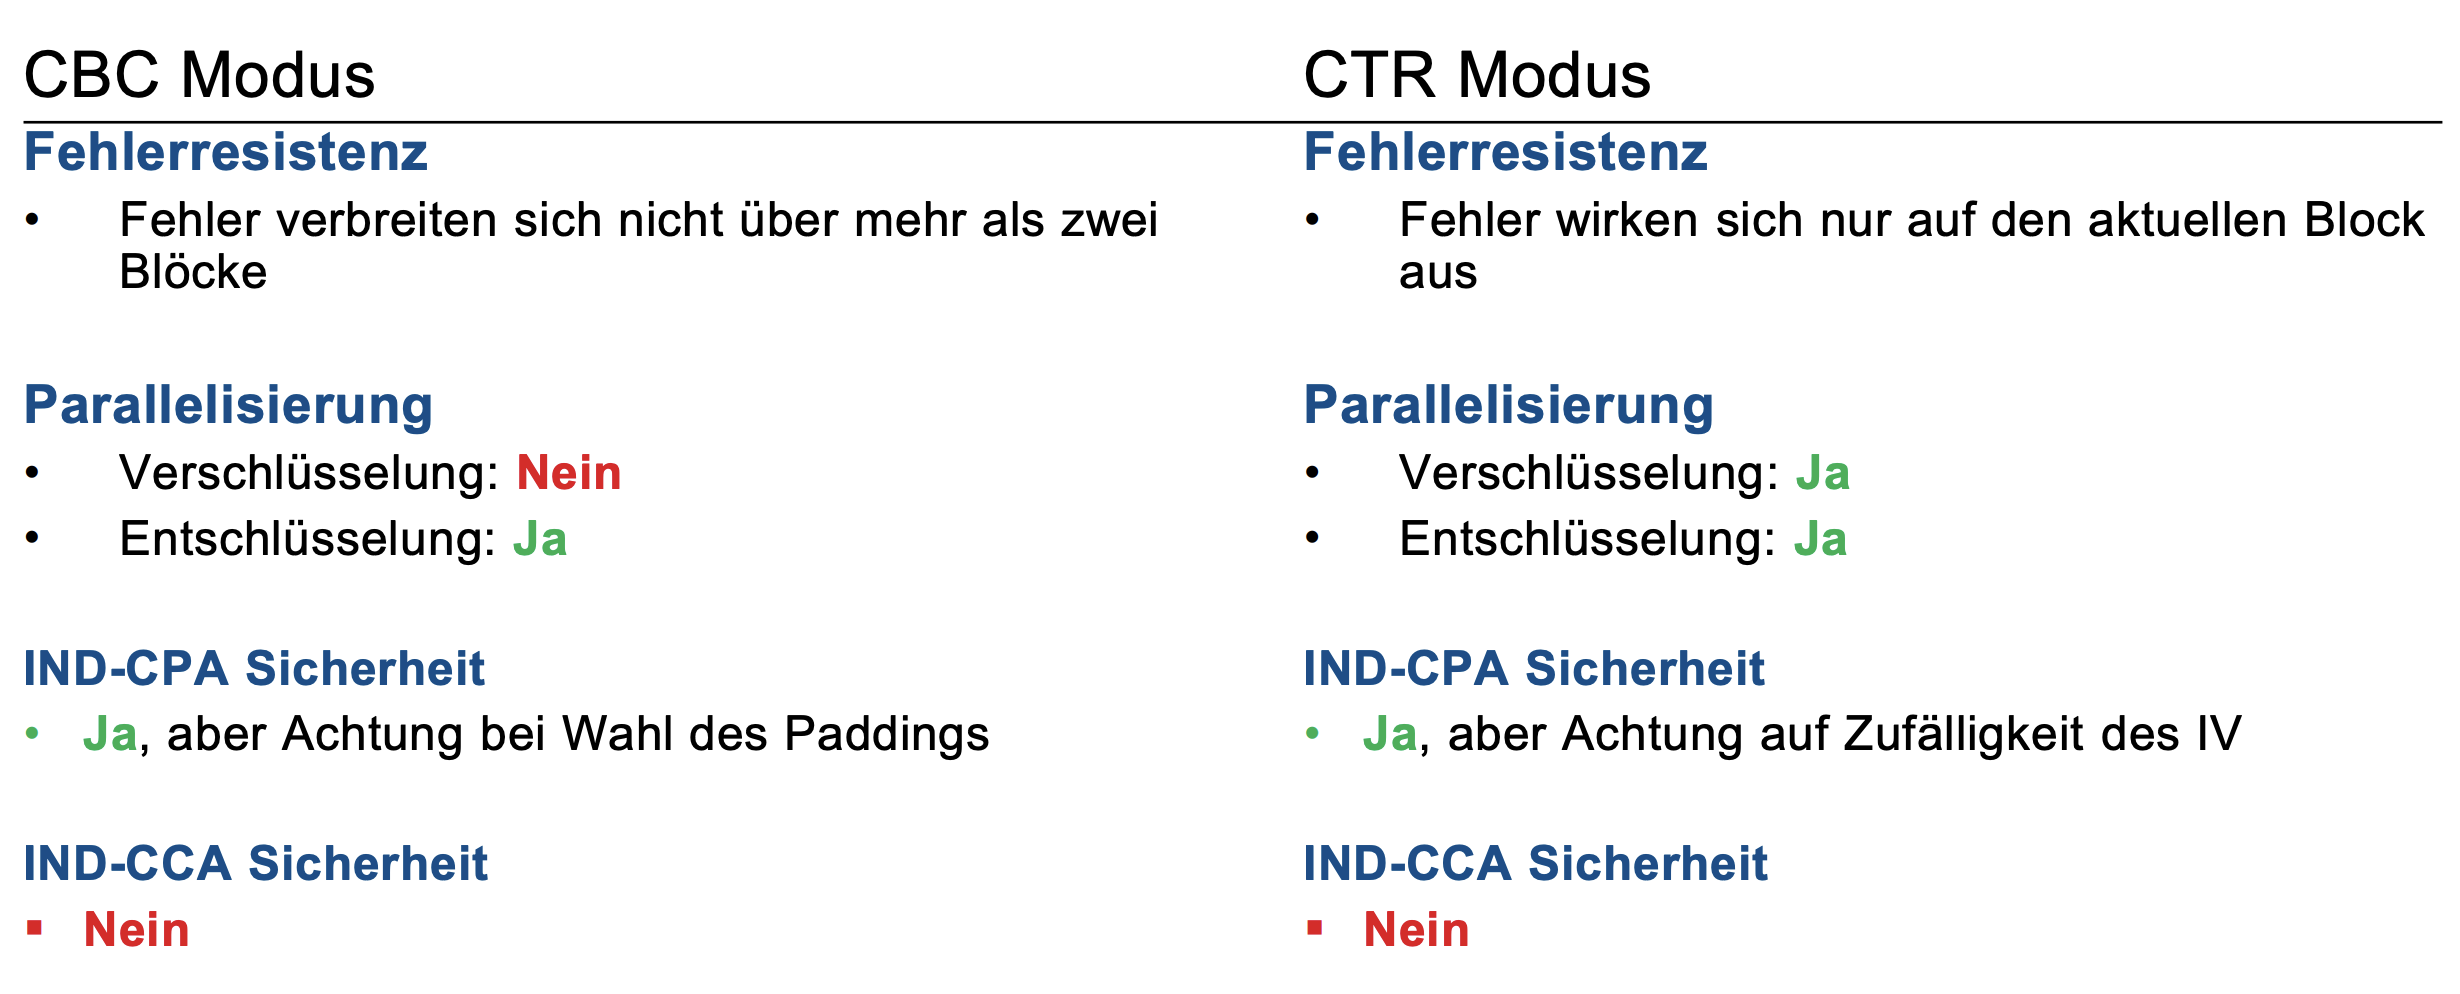
\includegraphics[width=0.7\linewidth]{/Users/lenavo/Desktop/3.Semester/Computersystemsicherheit/img/vergl.png}
    \caption{Vergleich der unterschiedlichen Modi}
    \label{fig:enter-label}
\end{figure}
\subsection{Kryptographische Hashfunktionen}
\subsubsection{Hashfunktionen}
\begin{itemize}
    \item Eingabe von Nachrichten mit \textbf{beliebiger Länge}
    \item Ausgabe mit \textbf{fixer Länge} ("message digest")
    \item Determinismus: selbe Eingabe erzeugt immer denselben Hashwert
\end{itemize}

$H: \{ 0,1\}^* \rightarrow \{ 0,1\}^n$ bildet von großer Definitionsmenge auf kleineren Bildbereich ab
\subsubsection{Sicherheitsdefinitionen}
\begin{figure}[h]
    \centering
    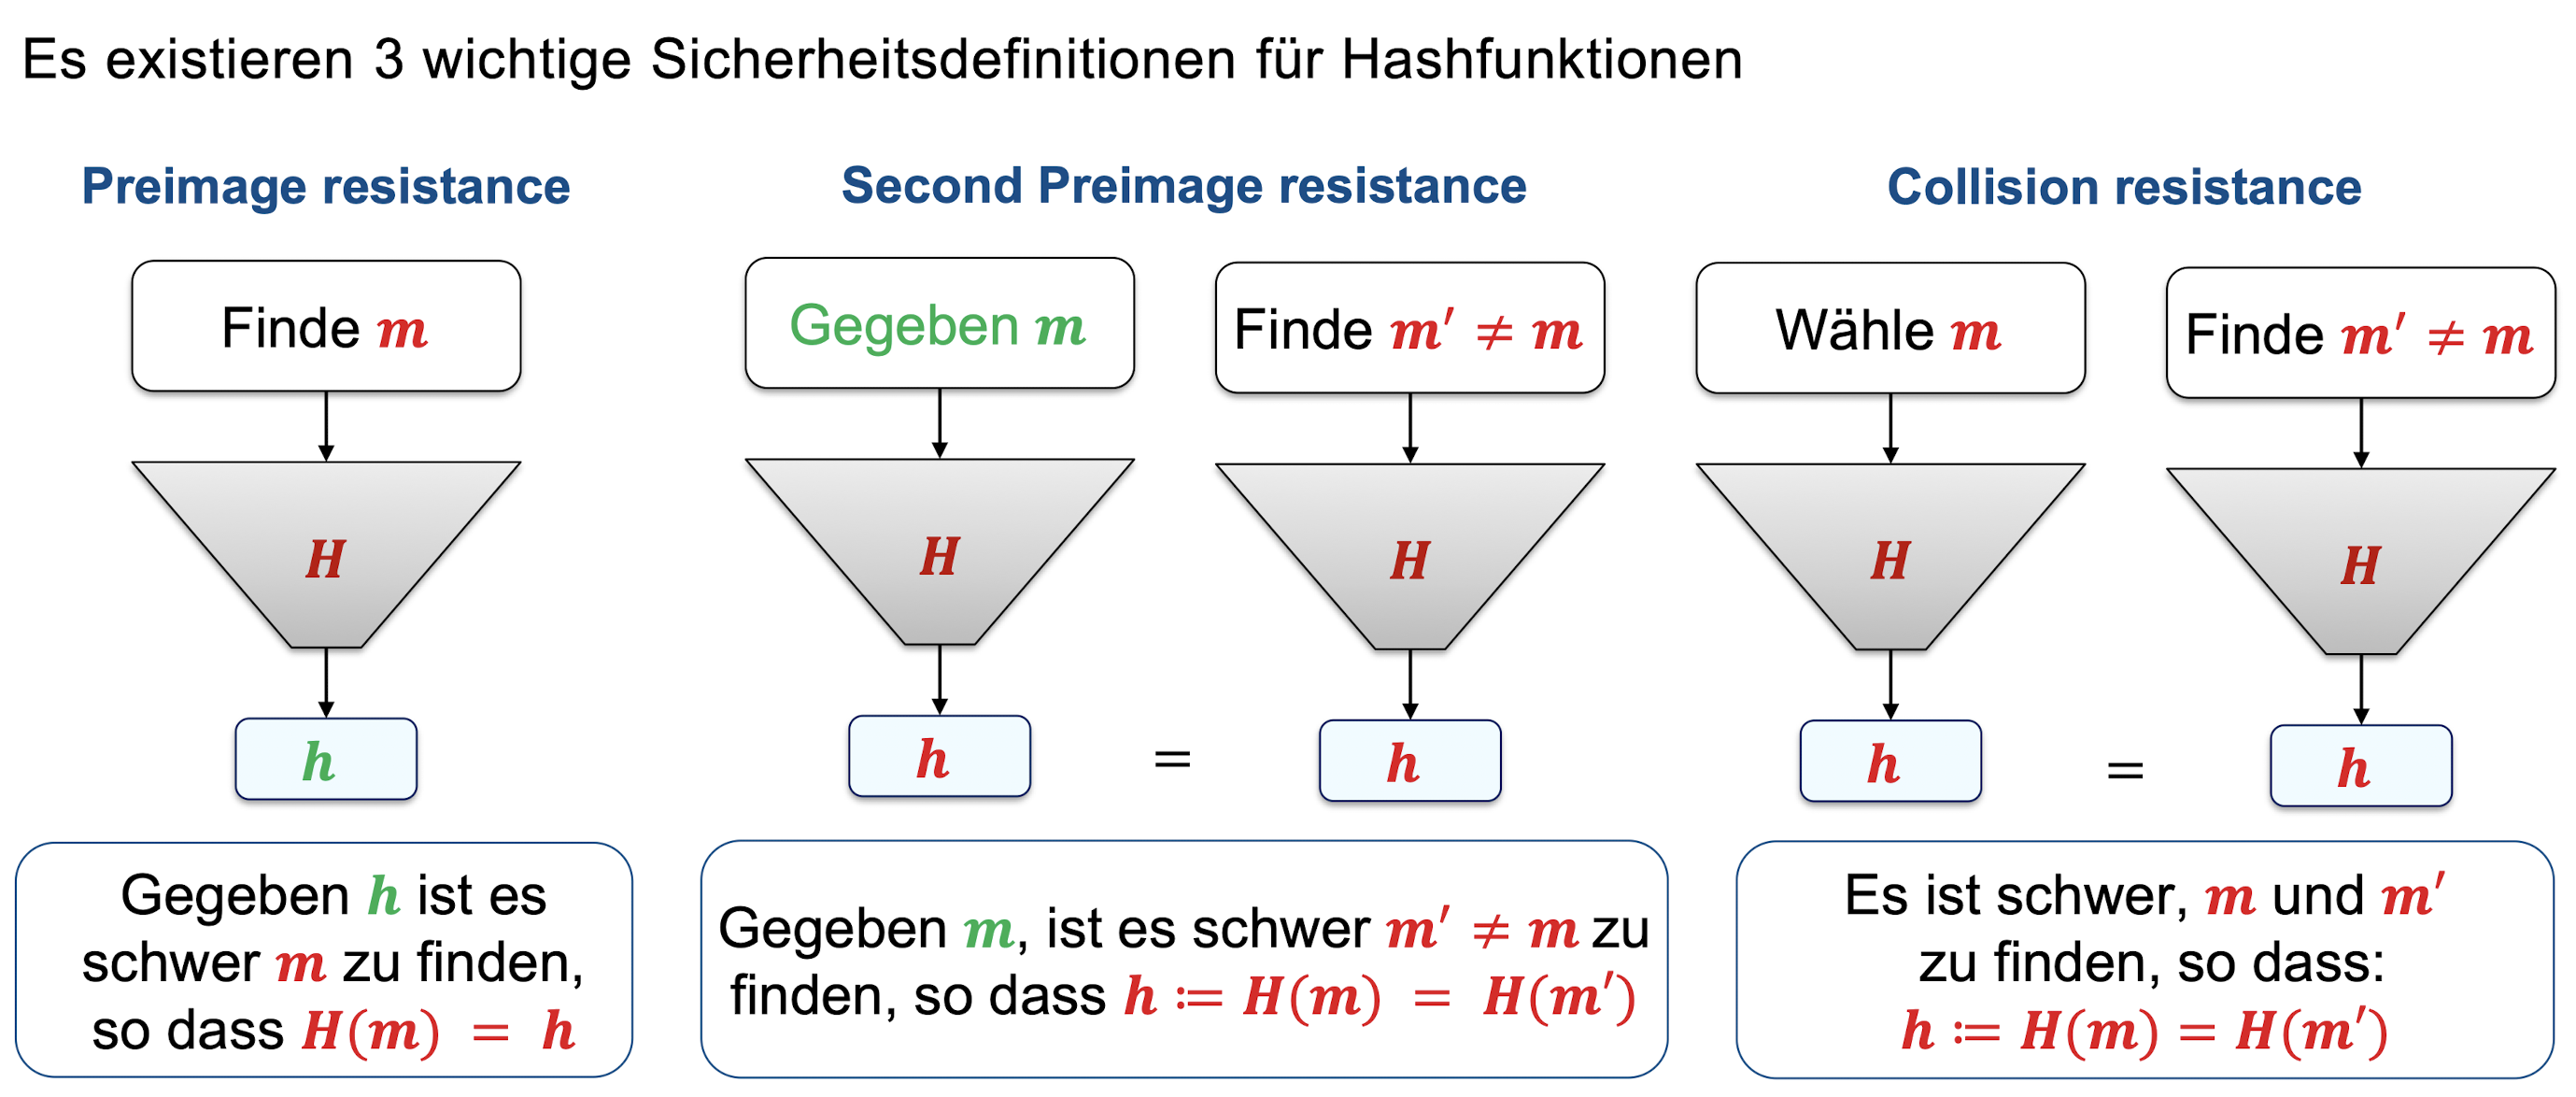
\includegraphics[width=0.7\linewidth]{/Users/lenavo/Desktop/3.Semester/Computersystemsicherheit/img/sicherheitsdef.png}
    \caption{Sicherheitsdefinitionen}
    \label{fig:enter-label}
\end{figure}

\noindent\textbf{Warum diese Sicherheitsdefinitionen?}\\[1.5mm]
\hl{Preimage Resistance (Urbildresistenz):}
\begin{itemize}
    \item diese Eigenschaft stellt sicher, dass es \textbf{extrem schwierig} ist , die ursprüngliche Nachricht (oder Eingabe) aus einem gegebenen Hashwert zu \textbf{rekonstruieren}
    \item \textbf{Nutzen:} schützt vor Rekonstruktion aus Hash-Wert, z.B. um Vertraulichkeit von Passwörtern zu sichern
\end{itemize}
\hl{Second Preimage Resistance (Zweite Urbildresistenz):}
\begin{itemize}
    \item diese Eigenschaft schützt davor, dass ein Angreifer, der eine Nachricht $m$ kennt, eine andere Nachricht $m'$ findet, die denselben Hash-Wert hat wie $m$
    \item \textbf{Nutzen:} Verhindert Finnden verschiedener Daten mit gleichem Hash-Wert, z.B. schwierig zwei gültige Zertifikate zu erzeugen
\end{itemize}

\noindent\hl{Collision Resistance (Kollisionsresistenz):}
\begin{itemize}
    \item diese Eigenschaft stellt sicher, dass es extrem schwierig ist, zwei beliebige unterschiedliche Nachrichten $m$ und $m'$ zu finden, die denselben Hash-Wert haben
    \item \textbf{Nutzen:} Kollisionen sind ausgeschlossen und damit für beliebige Anwendungen anwendbar
\end{itemize}

\subsection{Message Authentication Codes}
\begin{itemize}
    \item  kryptografisches Verfahren, das sicherstellt, dass eine Nachricht während der Übertragung \textbf{nicht manipuliert wurde und tatsächlich vom angegebenen Absender} stammt
    \item dient dazu, die \hl{Integrität und Authentizität} einer Nachricht zu garantieren, was für sichere Kommunikation essenziell ist
\end{itemize}
\newpage
\begin{figure}[h]
    \centering
    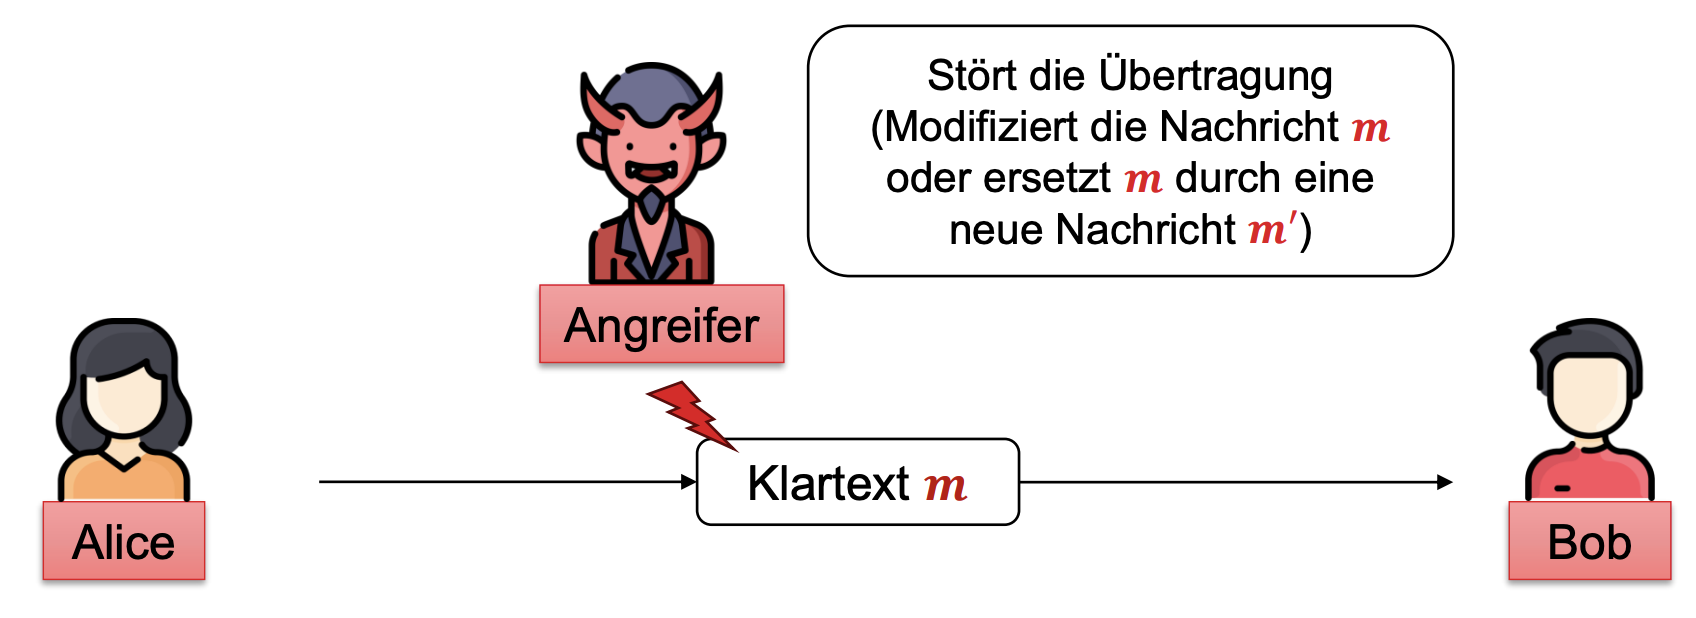
\includegraphics[width=0.6\linewidth]{/Users/lenavo/Desktop/3.Semester/Computersystemsicherheit/img/mac.png}
    \caption{Message Authentication}
    \label{fig:enter-label}
\end{figure}
\begin{itemize}
    \item Im Allgemeinen garantiert Verschlüsselung allein \textbf{nicht die Integrität} einer Nachricht
    \item schützt lediglich die Vertraulichkeit der Daten, jedoch nicht deren Unverfälschheit
\end{itemize}
\textbf{Was wird benötigt?}
\begin{itemize}
    \item \hl{Gen (Key-Generation)}
    \begin{itemize}
        \item generiert einen geheimen Schlüssel $k$ basierend auf einem Sicherheitsparameter
    \end{itemize}

    \item \hl{Mac (Tag-Generierung)}
    \begin{itemize}
        \item berechnet einen Authentifizierungstag $t$ basierend auf der Nachricht $m$ und dem Schlüssel $k$
    \end{itemize}

    \item \hl{Vrfy (Verifikation)}
    \begin{itemize}
        \item überprüft die Gültigkeit eines Tags $t$ für die Nachricht $m$ und den Schlüssel $k$
    \end{itemize}
\end{itemize}
\begin{figure}[h]
    \centering
    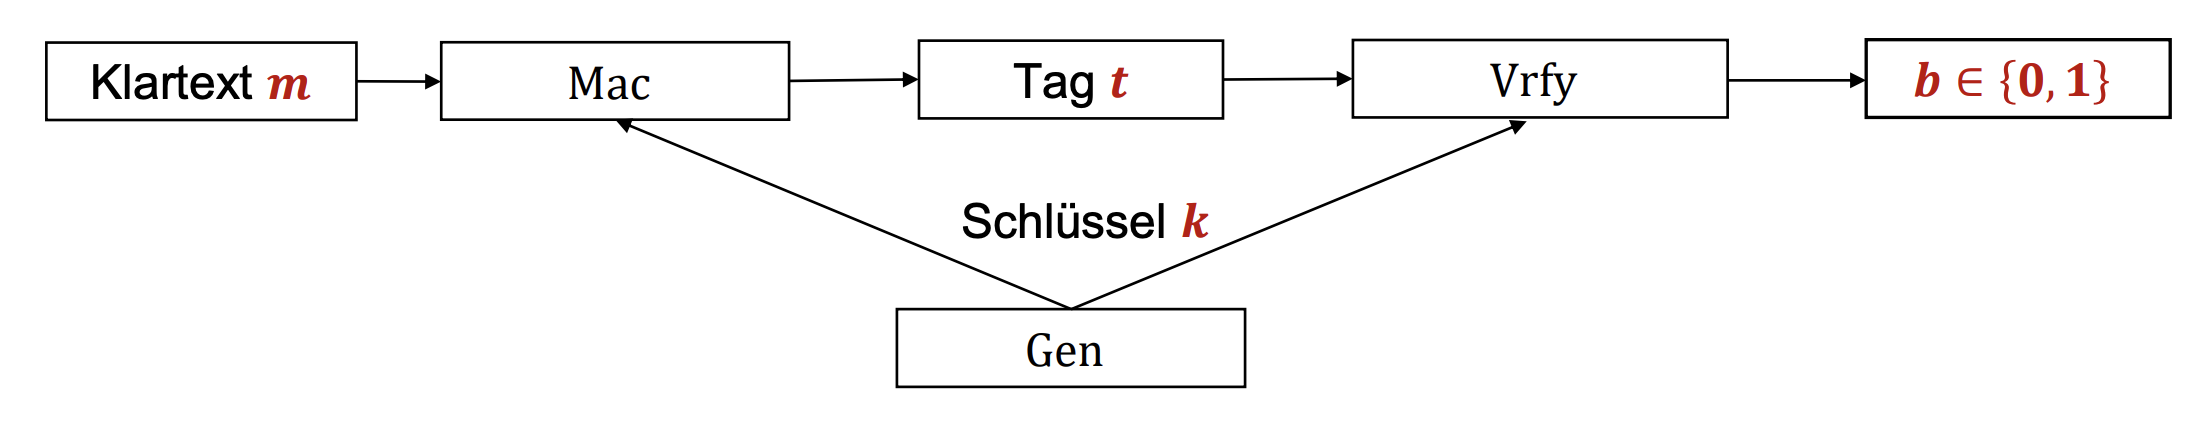
\includegraphics[width=0.6\linewidth]{/Users/lenavo/Desktop/3.Semester/Computersystemsicherheit/img/macs.png}
    \caption{Message Authentication Code}
    \label{fig:enter-label}
\end{figure}
\textbf{Korrektheit:}
Die Verifizierung eines gültigen Tags $t$ für eine Nachricht $m$ und dem Schlüssel $k$ muss korrekt sein. Das bedeutet:
\begin{equation}
    Vrfy_k(m, Mac_k(m)) = 1
\end{equation}
\textbf{Effizienz:}
Authentifizierung und Verifizierung sind effizient ($>$10 GB/s)
\subsubsection{Sicherheitsdefinition}
\begin{itemize}
    \item Ziel des Angreifers: Was ist ein erfolgreicher Angriff?
    \begin{itemize}
        \item naive Option: Angreifer lernt den Schlüssel k nicht
        \item in der Kyptographie: Angreider kann \textbf{keinen validen Tag} $t$ für $m$ erzeugen
    \end{itemize}
\end{itemize}
\textbf{Arten von MACs}
\begin{enumerate}
    \item \hl{Informationstheoretisch sichere MACs} $\longrightarrow$ \textbf{nicht effizient} für Authentifizierung von vielen Nachrichten
    \item \hl{Komplextheoretisch sichere MACS}
    \begin{itemize}
        \item für Nachrichten \textbf{fixer} Länge
        \item für Nachrichten mit \textbf{beliebiger} Länge, z.B. \textbf{CBC-MAC} und \textbf{HMAC}
    \end{itemize}
\end{enumerate}
\subsubsection{CBC-MAC}
\begin{itemize}
    \item ist ein Verfahren zur Berechnung eines \textbf{Message Authentication Codes (MAC)} auf Basis einer Blockchiffre
    \item veerwendet den \textbf{CBC-Modus}, um eine Nachricht zu authentifizieren
    \item der resultierende Tag (MAC-Wert) wird aus dem letzten Block des \textbf{CBC-Verschlüsselungsprozesses abgeleitet}
\end{itemize}
\textbf{Funktionsweise von CBC-MAC:}
\begin{enumerate}
    \item Sei $F_k: \{0,1\} \text{x} \{0,1\}^n \longrightarrow \{0,1\}^n$ eine Blockchiffre mit Schlüssel $k$, die Blöcke der Länge $n$ verarbeitet 
    \item die Nachricht $m$ wird in \textbf{gleich große Blöcke} aufgeteilt: $m = (m_1, m_2,\dots,m_t)$, wobei jeder Block $m_i \in \{0,1\}^n$ ist
    \item der \textbf{Initialisierungsvektor} (IV) wird aud $0^n$ gesetzt (eine Nullfolge der Länge n)
    \item die Blöcke der Nachricht werden \textbf{iterativ} mit der Blockchiffre im CBC-Modus verarbeitet
    \begin{itemize}
        \item der letzte Block wird als Tag ausgegeben
    \end{itemize}
    \item Prüfen ob Tag gültig ist: $ Vrfy_k (m,t): \tilde{t}  = \text{CBC} - MAC_k (m)$
    \begin{itemize}
        \item gib 1 aus, dalls $t = \tilde{t}$, ansonsten 0
    \end{itemize}
\end{enumerate}
\textbf{Wichtig:} CBC-MAC ist nur \textbf{sicher für Nachrichten mit fester Länge}
\begin{figure}[h]
    \centering
    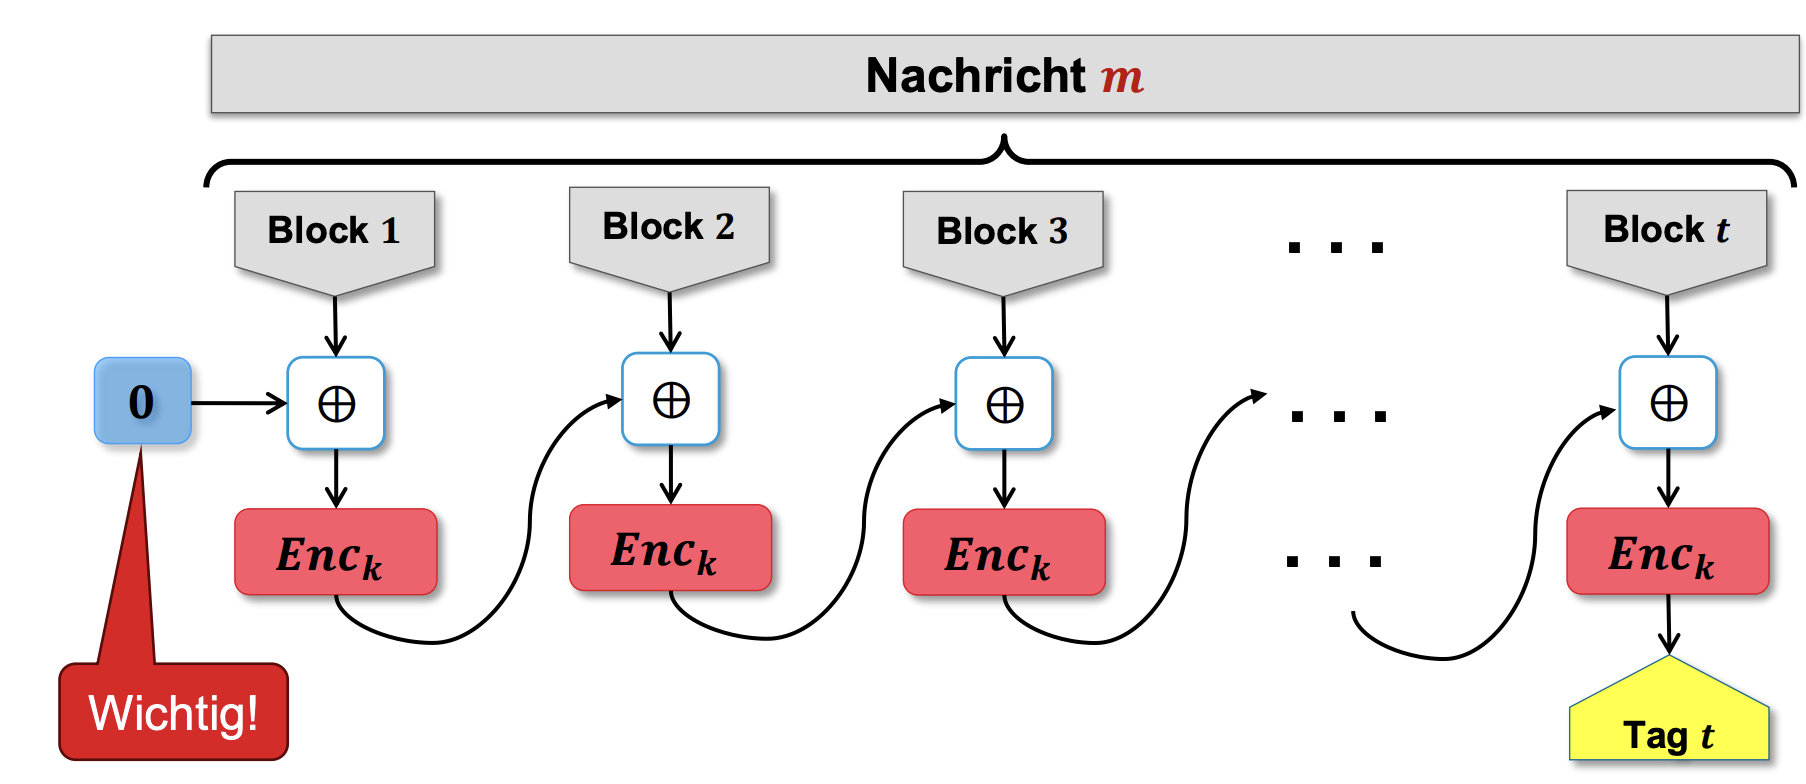
\includegraphics[width=0.6\linewidth]{/Users/lenavo/Desktop/3.Semester/Computersystemsicherheit/img/cbc-mac.png}
    \caption{CBC-MAC}
    \label{fig:enter-label}
\end{figure}\\
\textbf{CBC-MAC mit Nachrichten unterschiedlicher Länge}
\begin{itemize}
    \item Nachrichten $m$ mit $CBC-MAC_k(m) = t$ und $m'$ mit $CBC-MAC_k(m) = t$
\end{itemize}
\begin{figure}[h]
    \centering
    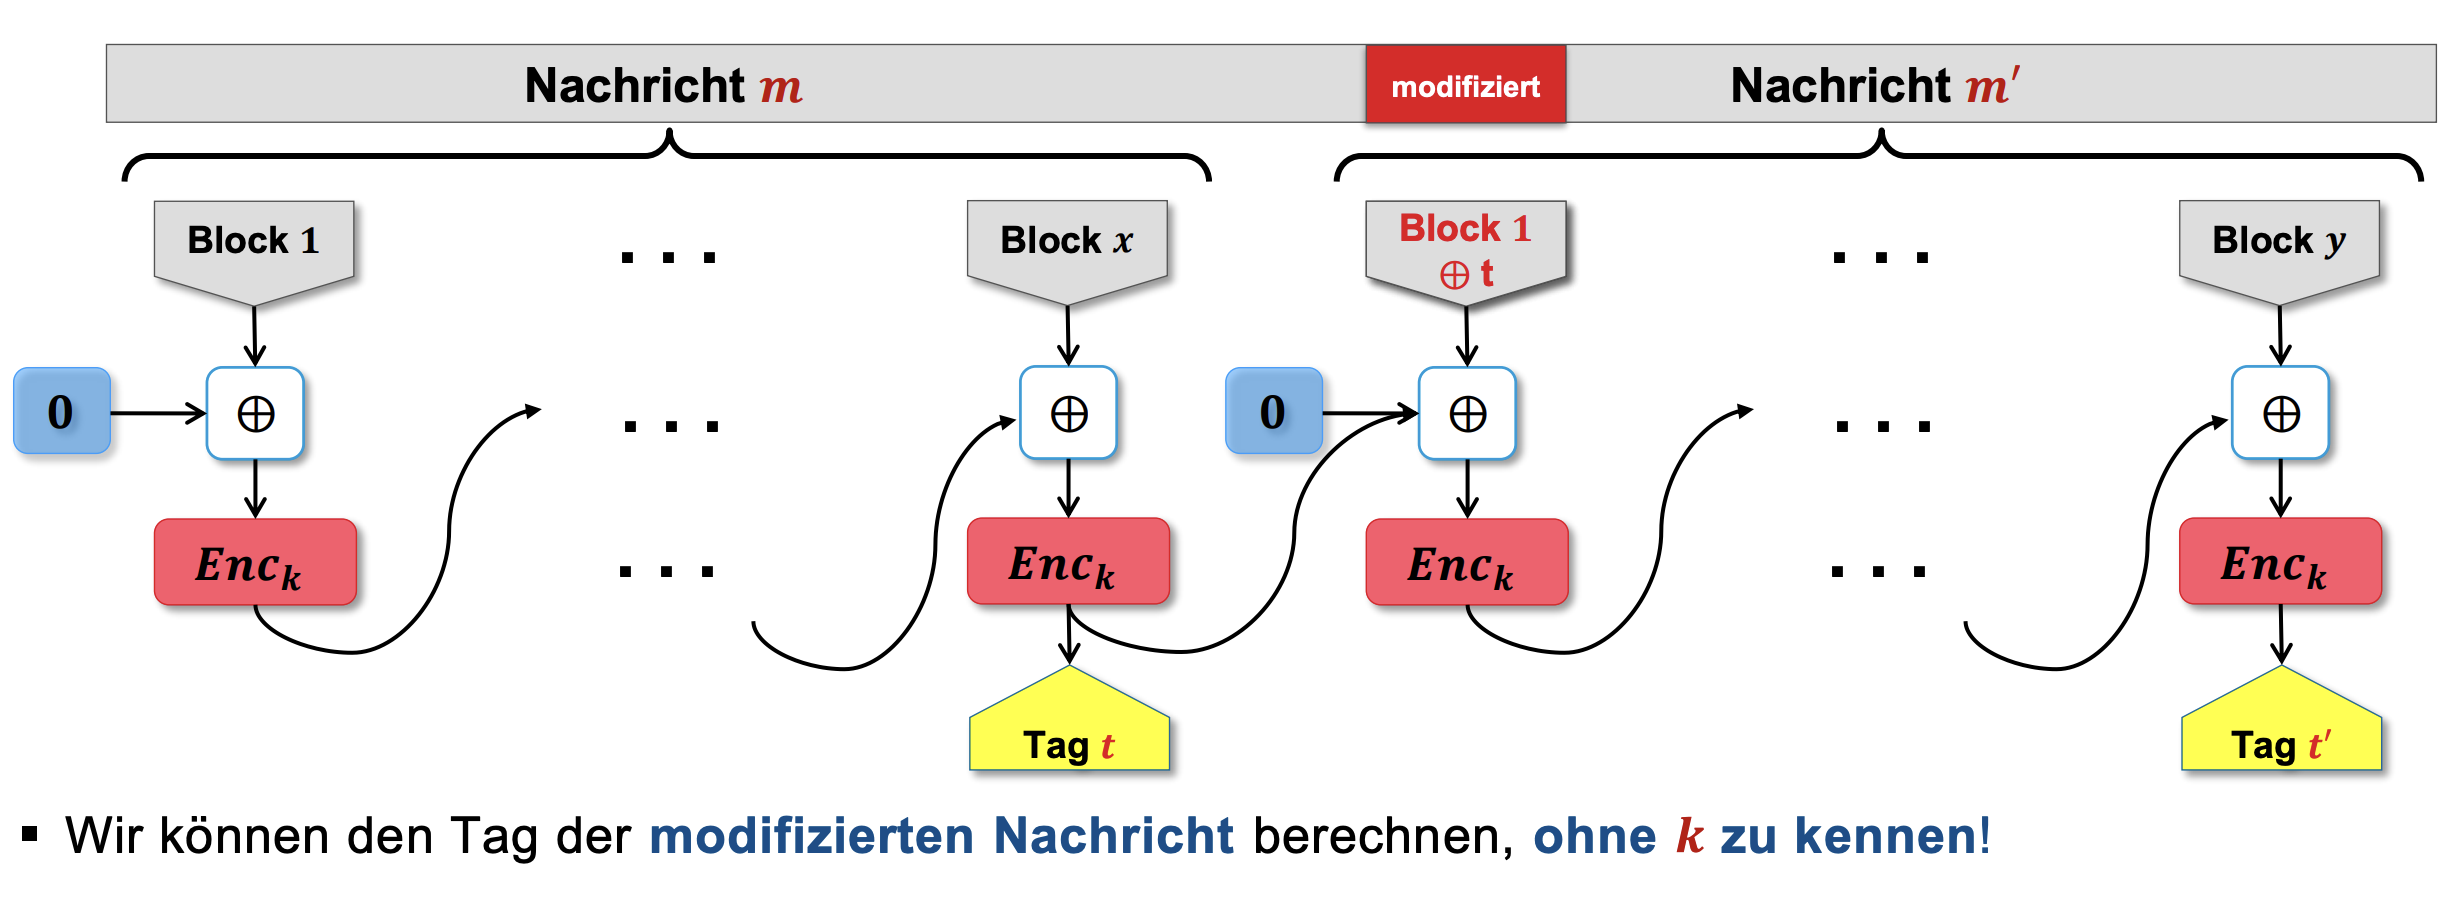
\includegraphics[width=0.7\linewidth]{/Users/lenavo/Desktop/3.Semester/Computersystemsicherheit/img/cbcmac.png}
    \caption{CBC-MAC - unterschiedliche Länge}
    \label{fig:enter-label}
\end{figure}

\subsubsection{Hash-und-MAC}
\hl{Konstruktionsidee:}
\begin{enumerate}
    \item Berechne $y = H(m)$ der langen Nachricht $m$ mit Hilfe von Domain-Extension für Hashfunktionen
    \item Berechne $MAC_k(y)$ mit MAC für fixe Nachrichtenlänge
\end{enumerate}

\begin{figure}[h]
    \centering
    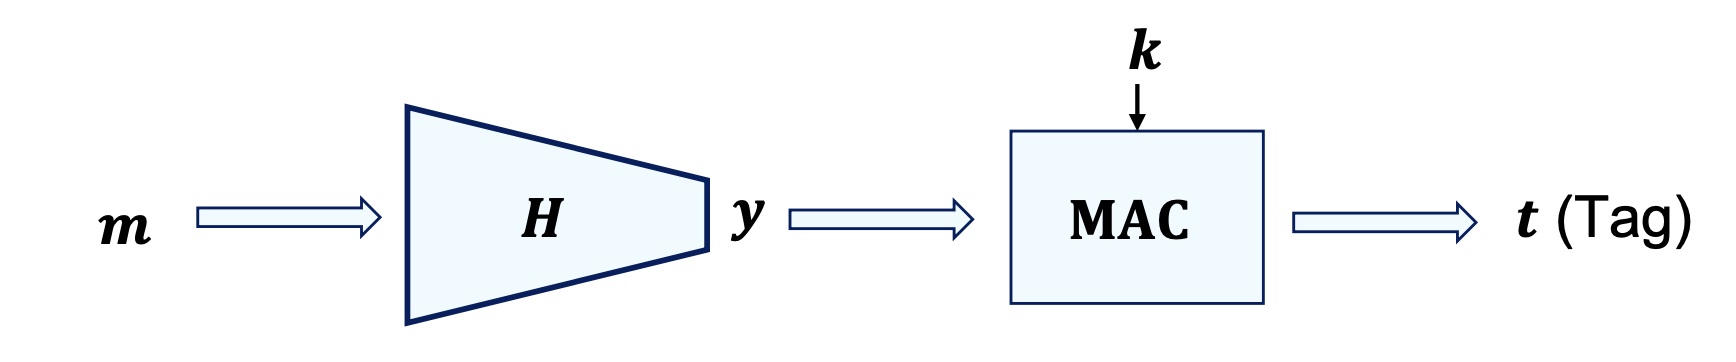
\includegraphics[width=0.7\linewidth]{/Users/lenavo/Desktop/3.Semester/Computersystemsicherheit/img/hashundmac.png}
    \caption{Hash-und-MAC}
    \label{fig:enter-label}
\end{figure}
\subsubsection{HMAC (Hash-based Message Authentication Code)}
\begin{itemize}
    \item sichere und flexible Konstruktion, die auf einer \textbf{Hashfunktion} basiert und zur \textbf{Authentifizierung von Nachrichten} verwendet wird
    \item \hl{Trivialer Ansatz:} $MAC_k (y) = H(k||y)$
    \item sicher für \textbf{manche Hash-Funktionen}, wie SHA-3, da diese nicht anfällig für bestimmte Angriffe sind
    \item unsicher für andere Hash-Funktionen, wie SHA-256
    \begin{itemize}
        \item arbeitet mit \textbf{fixen Eingabelängen} und \textbf{iterativem Hashing}
        \item trivialer Ansatz ist anfällig für \textbf{length extension attacks}
    \end{itemize}
\end{itemize}
\textbf{Bessere Lösung: HMAC (RFC 2014)}
\begin{itemize}
    \item umgeht Probleme des trivialen Ansatzes durch eine robustere Konstruktion
    \item nutzt \hl{zwei Padding-Werte} (inner padding und outer padding)
\end{itemize}
\subsection{Authentifizierte Verschlüsselung}
\begin{itemize}
    \item kombiniert \textbf{Vertraulichkeit, Integrität} und \textbf{Authentizität} von Nachrichten
    \item stellt sicher, dass ein Angreifer weder Klartext einer Nachricht lesen, noch diese manipulieren kann
\end{itemize}
\subsubsection{Encrypt-then-MAC}
\begin{itemize}
    \item Nachricht wird zunächst \textbf{verschlüsselt} und anschließend der Chiffretext mit \textbf{MAC authentifiziert}
\end{itemize}
\begin{figure}[h]
    \centering
    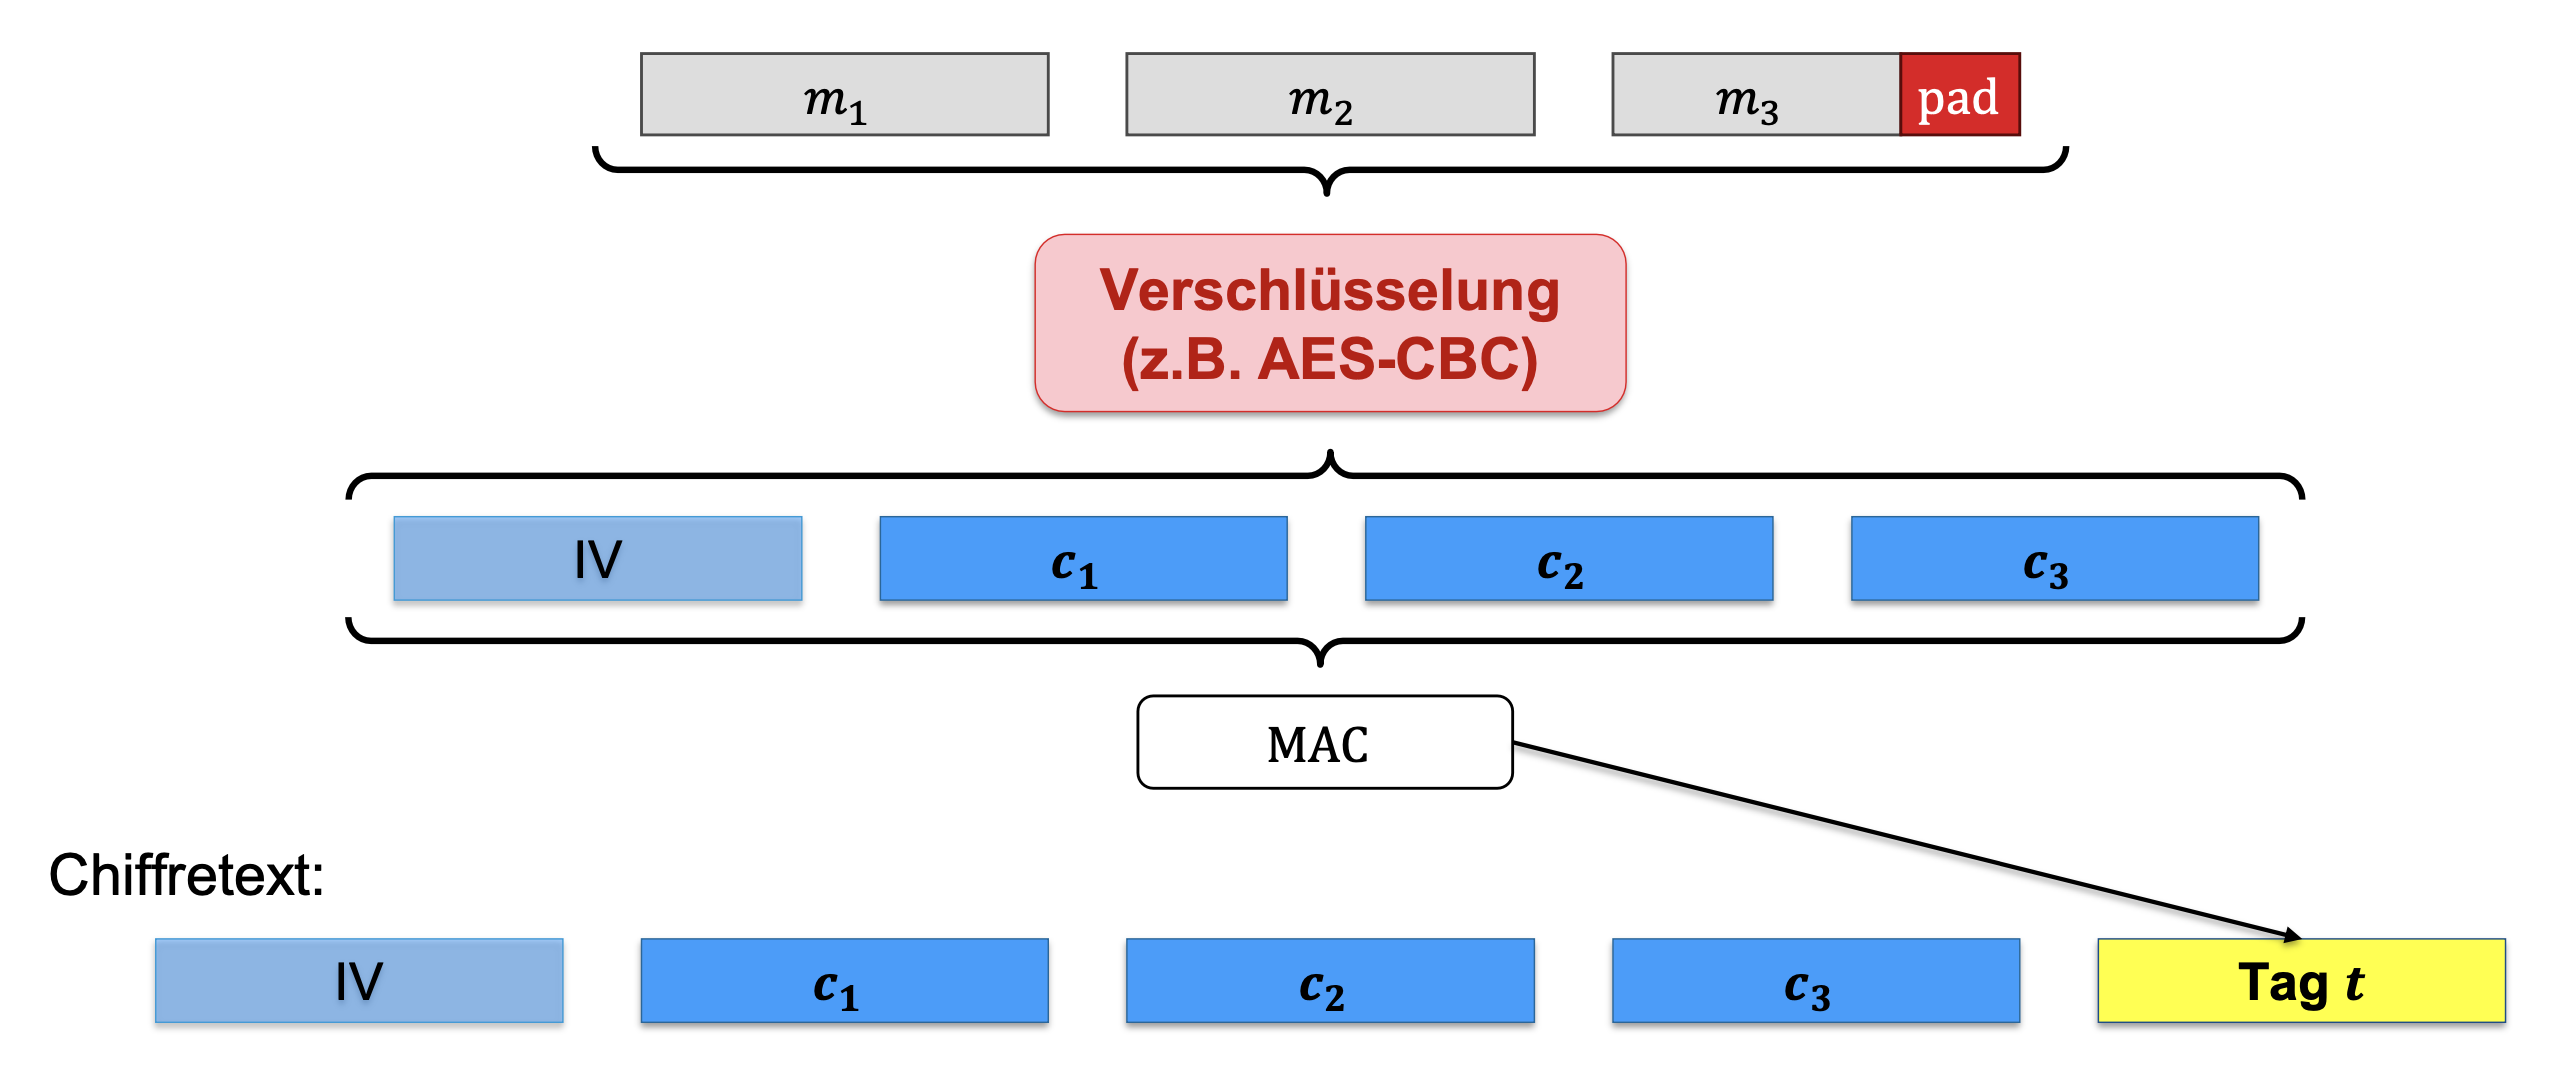
\includegraphics[width=0.5\linewidth]{/Users/lenavo/Desktop/3.Semester/Computersystemsicherheit/img/encrthenmac.png}
    \caption{Encrypt-then-MAC}
    \label{fig:enter-label}
\end{figure}

\subsubsection{Encrypt-then-MAC oder MAC-then-Encrypt}
\hl{Encrypt-then-MAC}
\begin{itemize}
    \item nur \textbf{authentische Chiffretexte} werden entschlüsselt
    \item beweisbar sicher 
    \item durch Authentifizierung auch \hl{IND-CCA sicher}
\end{itemize}

\noindent\hl{MAC-then-Encrypt}
\begin{itemize}
    \item die Nachricht wird \textbf{zuerst verschlüsselt}, und anschließend wird ein MAC über den Chiffretext berechnet 
    \item der Empfänger überprüft den MAC \textbf{vor der Entschlüsselung}
    \item wenn der MAC \textbf{ungültig} ist, wird die \textbf{Nachricht verworfen}, ohne dass eine Entschlüsselung stattfindet
    \item sicher gegen Padding Oracle-Angriffe, wie \hl{BEAST} und \hl{Lucky 13}
    \item nutzen Tatsache aus, dass auch dann entschlüsselt wird, falls Chiffretext verändert wurde
\end{itemize}
\end{document}





